%\documentclass[12pt]{report}
\documentclass[utf8, 14pt]{G7-32}  % ГОСТ 7.32-2001
%----------------------------------------------------------
% Значения констант по КП, НИРС, ВКР
%----------------------------------------%
% общие определения
\newcommand{\UpperFullOrganisationName}{Министерство науки и высшего образования Российской Федерации}
\newcommand{\ShortOrganisationName}{МГТУ~им.~Н.Э.~Баумана}
\newcommand{\FullOrganisationName}{федеральное государственное бюджетное образовательное\newline учреждение высшего профессионального образования\newline <<Московский государственный технический университет имени Н.Э.~Баумана\newline (национальный исследовательский университет)>> (\ShortOrganisationName)}
\newcommand{\OrganisationAddress}{105005, Россия, Москва, ул.~2-ая Бауманская, д.~5, стр.~1}
%----------------------------------------%
\newcommand{\gitlabdomain}{sa2systems.ru:88}
%----------------------------------------------------------
\newcommand{\doctypesid}{kp} % vkr (выпускная квалификационная работа) / kp (курсовой проект) / kr (курсовая работа) / nirs (научно-исследовательская работа студента) / nkr (научно-квалификационная работа)

% Тема должна быть сформулирована так, чтобы рассказать, о чем работа, но сделать это так, чтобы у читателя возникло желание читать аннота-цию. При формулировке темы не следует стараться рассказать о работе всё. Пример корректной темы: "Математическое моделирование процесса размножения медуз в Южно-Китайском море". Пример некорректной темы: "Применение модели SIS для моделирования процесса размножения медуз в Южно-Китайском море с использованием метода Рунге-Кутты и многопроцессорных вычислительных систем".
\newcommand{\Title}{Разработка web-приложения, обеспечивающего построение графовых моделей алгоритмов обработки данных}%{}
\newcommand{\TitleSource}{кафедра} % кафедра, предприятие, НИР, НИР кафедры, заказ организации

\newcommand{\SubTitle}{по дисциплине <<Модели и методы анализа проектных решений>>} % Методы оптимизации
\newcommand{\faculty}{<<Робототехника и комплексная автоматизация>>}
\newcommand{\facultyShort}{РК}
\newcommand{\department}{<<Системы автоматизированного проектирования (РК-6)>>}
\newcommand{\departmentShort}{РК-6}

\newcommand{\Author}{Журавлев~Н.В.}
\newcommand{\AuthorFull}{Журавлев~Николай~Вадимович}
\newcommand{\ScientificAdviserPosition}{доцент, к.ф.-м.н.}	% Должность научного руководителя
\newcommand{\ScientificAdviser}{Соколов~А.П.}	% Научный руководитель
%\newcommand{\ConsultantA}{@Фамилия~И.О.@}				% Консультант 1
%\newcommand{\ConsultantB}{@Фамилия~И.О.@}				% Консультант 2
\newcommand{\Normocontroller}{Грошев~С.В.}		% Нормоконтролёр
\newcommand{\group}{РК6-72Б}
\newcommand{\Semestr}{осенний семестр} % Например: осенний семестр или весенний семестр
\newcommand{\BeginYear}{2022}
\newcommand{\Year}{2023}
\newcommand{\Country}{Россия}
\newcommand{\City}{Москва}
\newcommand{\TaskStatementDate}{<<\underline{\textit{10}}>> \underline{октября} \Year~г.} %Дата выдачи задания

\newcommand{\depHeadPosition}{Заведующий кафедрой}		% Должность руководителя подразделения
\newcommand{\depHeadName}{А.П.~Карпенко}		% Должность руководителя подразделения

% Цель выполнения
\newcommand{\GoalOfResearch}{создать основу для построения/сохранения/накопления графовый моделей, описывающих тот или иной процесс обработки данных} % с маленькой буквы и без точки на конце

% Объектом исследования называют то, что исследуется в работе. Например, для указанной выше темы объектом может быть популяция медуз, но никак ни модель SIS, ни Южно-Китайское море, ни метод моделирования популяции медуз.
\newcommand{\ObjectOfResearch}{архитектура процессов обработки данных}

% Предмет исследований (уже чем объект, определяется, исходя из задач: формулируется как существительное, как правило, во множественном числе, определяющее "конкретный объект исследований" среди прочих в рамках более общего)
\newcommand{\SubjectOfResearch}{визуализатор графовых моделей}

% Основная задача, на решение которой направлена работа
\newcommand{\MainProblemOfResearch}{создание визуализатора графовых моделей, который должен описывать объект проектирования, который имеет какие-либо параметры, изменяемые в процессе обхода графа.}

% Выполненные задачи
\newcommand{\SubtasksPerformed}{%
В результате выполнения работы:
\begin{inparaenum}[1)]
	\item предложено создание визуализатора графовых моделей;
	\item создан алгоритм обхода ориентированного графа;
	\item разработано алгоритмы визуализации и обхода графа. Возможность чтения и вывод из файла формата aDot;
\end{inparaenum}}

% Ключевые слова (представляются для обеспечения потенциальной возможности индексации документа)
\newcommand{\keywordsru}{%
	ориентированные графы, обход графа, визуализация графа, aDot, web-приложение} % 5-15 слов или выражений на русском языке, для разделения СЛЕДУЕТ ИСПОЛЬЗОВАТЬ ЗАПЯТЫЕ
\newcommand{\keywordsen}{%
	@keywordsen@} % 5-15 слов или выражений на английском языке, для разделения СЛЕДУЕТ ИСПОЛЬЗОВАТЬ ЗАПЯТЫЕ

% Краткая аннотация
\newcommand{\Preface}{
Работа посвящена разработке визуализатора графовых моделей, с некоторыми особенностями. А именно, граф должен описывать объект проектирования, который имеет какие-либо параметры, которые должны изменяться в графе. Узлами графа является определенные значения параметров изучаемого объекта. В ребрах должен исполняться код на языке Python, предварительно занесённый туда пользователем. Этот код должен изменять какие-либо параметры объекта проектирования. При разработке для визуализации графа был использован алгоритм dot, а для обхода графа был создан собственный.
} % с большой буквы с точкой в конце

%----------------------------------------%
% выходные данные по документу
\newcommand{\DocOutReference}{\Author. \Title\xspace\SubTitle. [Электронный ресурс] --- \City: \Year. --- \total{page} с. URL:~\url{https://\gitlabdomain} (система контроля версий кафедры РК6)}

%----------------------------------------------------------


%----------------------------------------------------------
%общая преамбула для всех лабораторных - настройки общего вида оформления
%----------------------------------------------------------
\usepackage{amsfonts}
\usepackage{amsmath}
%\usepackage{MnSymbol}
%----------------------------------------------------------
\newcommand{\doclicense}{\includegraphics[width=0.09\textwidth]{doc-spec/by.eps}\xspace}%\ccShareAlike

\usepackage[T2A]{fontenc}
\usepackage[utf8]{inputenc}
% Переносы приходится выключать, т.к. при попытке прохождения нормоконтроля TestVkr будет воспринимать перенесённые слова как два слова.
%\usepackage[russian]{babel} %% это необходимо для включения переносов english
\usepackage{float}
\usepackage{rotating}
\usepackage{multirow}
\usepackage{pdflscape}
\usepackage{bm}
% необходимо для возможности копирования и поиска в готовом PDF
%\usepackage{cmap}
\usepackage{array}
\usepackage{multicol}
\usepackage{relsize}
\usepackage{booktabs}
% Пакет необходим для поддержки многострочного подчеркивания текста
\usepackage[normalem]{ulem}
%-------------------------
% определение атрибутов сборки Git
\usepackage[grumpy, maxdepth=6]{gitinfo2}
\renewcommand{\gitMark}{[git] \textbullet{} \gitBranch\,@\,\gitAbbrevHash{} \textbullet{} \gitAuthorName, \gitAuthorEmail (\gitAuthorIsoDate)}
%-------------------------
\newcommand{\authorSID}{\Year, \group, \Author, \pdftexbanner, \jobname}
%-------------------------
%\newcommand{\authorSIDheader}[1][white]{\begin{tabular}{c}\thepage\\[-6pt]\textcolor{#1}{\tiny\authorSID}\\[-6pt]\textcolor{#1}{\tiny\gitMark}\end{tabular}}
\newcommand{\authorSIDheader}{\thepage}
%-------------------------
%\newcommand{\authorSIDright}{\begin{tabular}{c}\tiny\authorSID\\\tiny\gitMark\end{tabular}}
\newcommand{\authorSIDright}{\textcolor{gray!10.0}{\tiny\gitMark}}
%-------------------------
% Сохранение метаданных в PDF об авторе документа
\usepackage{hyperxmp}
\usepackage{hyperref}
\hypersetup{%
    bookmarks=false,        % show bookmarks bar?
    pdftoolbar=true,        % show Acrobat’s toolbar?
    pdfmenubar=true,        % show Acrobat’s menu?
    pdffitwindow=false,     % window fit to page when opened
    pdfstartview={FitH},    % fits the width of the page to the window
    pdftitle={\Title},    	% title
    pdfauthor={\Author},    % author
%		pdfcopyright={Copyright © \Year, \Author. Все права защищены.},
		pdfcopyright={CC BY 4.0, \Year, \Author.},
		pdflicenseurl={http://creativecommons.org/licenses/by/4.0/},
    pdfsubject={\SubjectOfResearch},   % subject of the document
    pdfcreator={\pdftexbanner},   % creator of the document
%		pdfpublisher={Computer-aided design department, Bauman Moscow State Technical University},
		pdfcaptionwriter={Ass. Prof., PhD. Alexandr P. Sokolov},
    pdfproducer={\Author(\gitAuthorEmail), \group, \Year, Computer-aided design department, Bauman Moscow State Technical University}, % producer of the document
    pdfkeywords={\keywordsru, \keywordsen}, % producer of the document
    pdfnewwindow=true,      % links in new window
    colorlinks=true,
    citecolor=black,
    linkcolor=black,      % color of internal links (change box color with linkbordercolor)
    urlcolor=black,
    filecolor=black      % color of file links
}
%----------------------------------------------------------------
\usepackage{xspace}
%----------------------------------------------------------
%\usepackage[style=long4colheader, translate=babel, section=chapter, toc]{glossaries}
%\usepackage[abbreviations, toc=true, xindy, automake]{glossaries-extra}
%\setglossarystyle{treenoname}%+
%\makeglossaries

\usepackage[style=long, acronyms, nonumberlist, nomain, nogroupskip=true, translate=babel, section=chapter]{glossaries}
\usepackage[abbreviations, toc=false, automake=true]{glossaries-extra}

\renewenvironment{theglossary}{\begin{longtable}[l]{p{0.15\linewidth}p{0.8\linewidth}}}{\end{longtable}}
\newcommand{\listofacronymname}{Список сокращений и условных обозначений}
\newcommand{\listofdefinitions}{Словарь терминов}
\makeglossaries
%----------------------------------------------------------
% поддержка inparaenum
\usepackage{paralist}
%----------------------------------------------------------
% нужно для определения окружения description
%\usepackage{enumitem}
%----------------------------------------------------------------
% Настройки вставки PDF (для вставки, к примеру, направления на защиту, акта об отсутствии заимствования, рецензии)
\usepackage{pdfpages}
\includepdfset{turn=true,scale=0.95,pages=-,pagecommand={\pagestyle{fancy}}}
%----------------------------------------------------------
\usepackage{tikz}
\usetikzlibrary{tikzmark}
\usetikzlibrary{matrix,automata,graphs}
\usetikzlibrary{arrows,arrows.meta,positioning,trees}
%----------------------------------------------------------
% необходимо для возможности включать в имена включаемых файлов _
%\usepackage[strings]{underscore}
%----------------------------------------------------------
% добавление поддержки команды вывода текста на полях \marginnote
\usepackage{marginnote}
% добавление поддержки команды \color
\usepackage{xcolor}
%--------------------------------------------
% final - удаляет все всплывающие комментарии
\usepackage[author={Alexandr Sokolov},opacity=0.1]{pdfcomment}
%\usepackage[author={Alexandr Sokolov},opacity=0.1,final]{pdfcomment}
\newcommand{\messnote}[1]{\marginnote{\color[rgb]{1,0,0}\Huge\textbf{!}\pdfcomment{#1}}[-1.0cm]}
%----------------------------------------------------------
% Произвольная нумерация списков.
\usepackage{enumerate}
%----------------------------------------------------------
%\raggedbottom
%\textwidth=163mm
%\textheight=220mm
%\oddsidemargin=-0.5pt
%\footskip=30pt
%\topmargin=27pt
%\headheight=12pt
%\headsep=25pt
%\topskip=10pt
%\baselineskip=15pt
%\topmargin=-4mm
%----------------------------------------------------------
\tolerance 1414
\hbadness 1414
\emergencystretch 1.5em
\hfuzz 0.3pt
\widowpenalty=10000
\vfuzz \hfuzz
\raggedbottom
%----------------------------------------------------------
% Настройки колонтитулов
\usepackage{fancyhdr} % Headers and footers
\fancyhf{} % clear all headers and footers - equivalent to %\fancyhead{} and \fancyfoot{}
\renewcommand{\headrulewidth}{0.0pt}
\renewcommand{\footrulewidth}{0.0pt}
%\renewcommand{\chaptermark}[1]{\markboth{ \chaptername\ \thechapter }{}}
\renewcommand{\chaptermark}[1]{\markboth{}{}}
\fancyhead[C]{}
\fancyfoot[C]{\authorSIDheader}%[white]}
%\setlength{\headheight}{17pt}%

\pagestyle{fancy} % All pages have headers and footers
%----------------------------------------%
%Необходимо для того, чтобы при использовании команды \thispagestyle{plain} стиль plain был переопределён на этот
\fancypagestyle{plain}{%
\fancyhf{}% clear all header and footer fields
\renewcommand{\headrulewidth}{0pt}%
\renewcommand{\footrulewidth}{0pt}%
\fancyhead[C]{}
\fancyfoot[C]{\authorSIDheader}%[white]}
}
%----------------------------------------------------------
\usepackage[hpos=0.98\paperwidth, % .98 to prevent bleed
            vpos=0.7\paperwidth,
            angle=90]{draftwatermark}

\SetWatermarkText{\authorSIDright}
%\SetWatermarkColor[gray]{0.1}
\SetWatermarkFontSize{0.2cm}
\SetWatermarkAngle{90}
\SetWatermarkHorCenter{20cm}
%----------------------------------------------------------
% указание
\setcounter{secnumdepth}{2}
%----------------------------------------------------------
% Пакеты для подсчета количества: страниц, и т.д.
\usepackage{etoolbox}
\usepackage{totcount,assoccnt}
%----------------------------------------------------------

% суперсчетчики всего ! :-)
\regtotcounter{page}

\newtotcounter{ffigure}
\setcounter{ffigure}{0}
\def\oldfigure{} \let\oldfigure=\figure
\def\figure{\stepcounter{ffigure}\oldfigure}

\newtotcounter{ttable}
\setcounter{ttable}{0}
\def\oldtable{} \let\oldtable=\table
\def\table{\stepcounter{ttable}\oldtable}

\newtotcounter{cchapter}
\setcounter{cchapter}{0}
\def\oldchapter{} \let\oldchapter=\chapter
\def\chapter{\stepcounter{cchapter}\oldchapter}

\newtotcounter{eequation}
\setcounter{eequation}{0}
\def\oldequation{} \let\oldequation=\equation
\def\equation{\stepcounter{eequation}\oldequation}

\newtotcounter{bibcnt}
\setcounter{bibcnt}{0}
\def\oldbibitem{} \let\oldbibitem=\bibitem
\def\bibitem{\stepcounter{bibcnt}\oldbibitem}

%----------------------------------------------------------
% необходимо для работы команды \xspace (умный пробел после замены, осуществляемой некоторой командой в тексте)
\usepackage{xspace}
%----------------------------------------------------------
% необходимо для того, чтобы в окружениях enumerate можно было менять формат нумерации
%\usepackage{enumitem}
%----------------------------------------------------------
%Необходимо для сокращения размера шрифта подписей и сокращения отступов между рисунком и подписью к нему
\usepackage[margin=5pt,font={small, singlespacing}, labelfont={small}, justification=centering, labelsep=period]{caption}
\captionsetup{belowskip=0pt}
%----------------------------------------------------------
% подключение листингов и определение языков
\usepackage{listings}

\lstset
{%
		extendedchars=\true, % включаем не латиницу
		frame=tb, % рамка сверху и снизу
		escapechar=|, % |«выпадаем» в LATEX|
		xleftmargin=0.5cm,
		xrightmargin=0.5cm,
		columns=fullflexible,
%		aboveskip=5pt,
		numbers=left,                    % where to put the line-numbers; possible values are (none, left, right)
		numbersep=4pt,                   % how far the line-numbers are from the code
		showspaces=false,
		showstringspaces=false,
		breakatwhitespace=true,         % sets if automatic breaks should only happen at whitespace
		breaklines=true,                 % sets automatic line breaking
		basicstyle=\color{black}\small\sffamily,%\ttfamily,% \sffamily
		commentstyle=\color{gray}\itshape, % шрифт для комментариев
		stringstyle=\color{orange},
%		stringstyle=\bfseries, % шрифт для строк
		numberstyle=\footnotesize\color{gray},
%		numberstyle=\ttfamily\small\color{gray}, % the style that is used for the line-numbers
		keywordstyle=\color{blue}\bfseries,
%		directivestyle=\color{red},
%		emph={int,char,double,float,unsigned,bool,string},
		emphstyle={\color{blue}\bfseries},
		tabsize=2,
%		morecomment=[l]{//},
%		otherkeywords={=,==,:,&},
		texcl=true,
}

\lstloadlanguages{Python, C++}

%--------------------------------------------
% необходимо для команды \cancelto{0}{x}
\usepackage{cancel}
%----------------------------------------------------------
% необходимо для того, чтобы доопределить спецификатор P, для
% использования в таблицах при форматировании
\usepackage{array}
\newcolumntype{P}[1]{>{\centering\arraybackslash}p{#1}}
%----------------------------------------%
% необходимо для того, чтобы допускались разрывы страниц внутри align align*
\allowdisplaybreaks
%----------------------------------------%
\makeatletter
\def\dynscriptsize{\check@mathfonts\fontsize{\sf@size}{\z@}\selectfont}
\makeatother
\def\textunderset#1#2{\leavevmode
  \vtop{\offinterlineskip\halign{%
    \hfil##\hfil\cr\strut#2\cr\noalign{\kern-.3ex}
    \hidewidth\dynscriptsize\strut#1\hidewidth\cr}}}

\newcommand\executer[1]{\textunderset{\scriptsize{подпись, дата}}{\signvrule} #1}
%----------------------------------------------------------
% необходимо для поддержки поворотов текста
\usepackage[absolute]{textpos}
\setlength{\TPHorizModule}{30mm}
\setlength{\TPVertModule}{\TPHorizModule}
\textblockorigin{0mm}{25mm} % start everything near the top-left corner
%----------------------------------------------------------
% оформление "теорем"
\usepackage{amsthm}
\usepackage{thmtools}
%----------------------------------------------------------
\newtheoremstyle{theoremstyle}% <name>
{0pt}% <Space above>
{0pt}% <Space below>
{\normalfont}% <Body font>
{0pt}% <Indent amount>
{\bfseries}% <Theorem head font>
{.}% <Punctuation after theorem head>
{.5em}% <Space after theorem headi>
{}% <Theorem head spec (can be left empty, meaning `normal')>
%----------------------------------------------------------
\theoremstyle{theoremstyle}

%\declaretheoremstyle[
  %headfont=\normalfont\bfseries,
%%	numberwithin=section,
  %bodyfont=\normalfont,
  %spaceabove=1em plus 0.75em minus 0.25em,
  %spacebelow=1em plus 0.75em minus 0.25em,
  %qed={$\blacksquare$},
	%headpunct={\newline},
%%  qed={$\square$},
%]{taskstyle}
%
%\declaretheorem[
  %style=taskstyle,
  %title=Задача,
  %refname={задача,задачи},
  %Refname={Задача,Задачи}
%]{task}
%
%\declaretheoremstyle[
  %headfont=\normalfont\bfseries,
	%numberwithin=task,
  %bodyfont=\normalfont,
  %spaceabove=1em plus 0.75em minus 0.25em,
  %spacebelow=1em plus 0.75em minus 0.25em,
	%headpunct={\newline},
%%  qed={$\blacksquare$},
  %qed={$\square$},
%]{variantstyle}
%
%\declaretheorem[
  %style=variantstyle,
  %title=Вариант,
  %refname={вариант,варианты},
  %Refname={Зариант,Варианты}
%]{variant}

%----------------------------------------------------------
%\newtheorem{question}{Вопрос}
%\newtheorem{task}{Задача}
%\newtheorem{solution}{Решение}
\newtheorem{remark}{Замечание}
\newtheorem{description}{Описание}
%%----------------------------------------------------------

%----------------------------------------------------------
\pdfminorversion=7
%----------------------------------------------------------
% общие вспомогательные определения
%----------------------------------------------------------
\def\argmax{\operatornamewithlimits{argmax}}
\DeclareMathOperator{\pr}{pr}
%\def\sgn{\operatornamewithlimits{sgn}}
\def\FEspoon{\ensuremath{\mathbin{\bullet\kern-0.2em{-}\kern-0.2em\circ}}}
\let\filledemptyspoon\FEspoon
\newcommand{\mbf}[1]{\boldsymbol{#1}}

%----------------------------------------------------------
% горизонтальная линия для последующего проставления подписи
\newcommand{\signhrule}{\raggedright\baselineskip0.0ex \vrule height 0.5pt width30mm depth0pt}
% место для проставления даты
\newcommand{\datetofill}{<<\uline{\textcolor{white}{\hspace{30pt}}}>>~\uline{\textcolor{white}{\hspace{80pt}}}~\Year~\cyrg.}

% 1 - role	% роль
% 2 - ФИО 	% подпись, дата
\newcommand{\signerline}[3][black]{%
#2 & \textunderset{подпись, дата}{\underline{\textcolor{white}{\hspace{120pt}}}} & & \textunderset{ФИО}{\uline{\textcolor{#1}{#3}}}  %фамилия, и.о.
}
%----------------------------------------------------------
\newcommand{\headerruleseparator}{%
\vrule height 0.6mm width 1.0\textwidth depth0pt
\vspace{-19pt}
\vrule height 0.2mm width 1.0\textwidth depth0pt
}
%----------------------------------------------------------
% 1 -- \depHeadPosition
% 2 -- \department
% 3 -- \depHeadName
\newcommand{\officialheader}{%
\begin{center}
\UpperFullOrganisationName\newline \FullOrganisationName
\end{center}
\vspace{-20pt}
\headerruleseparator}
%----------------------------------------------------------
% 1 -- \depHeadPosition
% 2 -- \department
% 3 -- \depHeadName
\newcommand{\signerblock}[3]{%
\parbox[t]{72.0mm}{%
\begin{center}
УТВЕРЖДАЮ\\
\vskip1.0mm
#1 \textunderset{индекс}{\underline{\textit{#2}}}\\%\newline
\vskip1.0mm
\textunderset{}{\signhrule} \quad \textit{#3}\newline
\datetofill
\end{center}
}}
%----------------------------------------------------------
\newcommand{\groupblock}[3]{%
\begin{tabular}{p{0.18\textwidth}p{0.15\textwidth}}
\hfill ФАКУЛЬТЕТ & \underline{#1} \\
\hfill КАФЕДРА & \underline{#2} \\
\hfill ГРУППА & \underline{#3} \\
\end{tabular}}
%-------------------------
\usepackage{ifthen}
\usepackage{calc}
%-------------------------
% #1 - showleft
% #2 - subdocname
% #3 - subdocnamedscra
\newcommand{\officialheaderfull}[3][]{%
\officialheader

\begin{center}
\vspace{-50pt}
\begin{tabular}{P{0.25\textwidth}P{0.3\textwidth}P{0.4\textwidth}}
\ifthenelse{\equal{#1}{showleft}}{\smash{%
		\raisebox{-1.25\height}{%
		\groupblock{\facultyShort}{\departmentShort}{\group}
		}}}{}
& & \signerblock{\depHeadPosition}{\departmentShort}{\depHeadName} \\
\end{tabular}
\end{center}

\begin{center}
\vspace{-15pt}
\large
\MakeUppercase{\textbf{#2}}\\
\textbf{#3}
\end{center}

\noindent\begin{tabular}{p{0.95\textwidth}}
Студент группы: \underline{\group} \\
\AuthorFull \\%[-10pt]
\hline
\multicolumn{1}{P{0.9\textwidth}}{\smaller[2] \vspace{-19pt}(фамилия, имя, отчество)}
\end{tabular}

\noindent%\begin{tabular}{p{0.95\textwidth}}
Тема \doctypec: \expandafter\uline\expandafter{\Title}% \\%[-10pt]
%\hline \\
%\end{tabular}
}
%-------------------------
% #1 - current \doctype
% #2 - destination document
% #3 - text
\newcommand{\myconditionaltext}[3]{%
\ifthenelse{\equal{#1}{kr}\AND\equal{#2}{kr}}{#3}{}%
\ifthenelse{\equal{#1}{kp}\AND\equal{#2}{kp}}{#3}{}%
\ifthenelse{\equal{#1}{vkr}\AND\equal{#2}{vkr}}{#3}{}%
\ifthenelse{\equal{#1}{nirs}\AND\equal{#2}{nirs}}{#3}{}%
\ifthenelse{\equal{#1}{nkr}\AND\equal{#2}{nkr}}{#3}{}%
}
% использование
%\myconditionaltext{\doctypesid}{kp}{XXXXXXX} % вставится только при сборке КП
%-------------------------
% к \doctypeb
\newcommand{\doctypeb}{%
\ifthenelse{\equal{\doctypesid}{vkr}}{выпускной квалификационной работе}{}%
\ifthenelse{\equal{\doctypesid}{kr}}{курсовой работе}{}%
\ifthenelse{\equal{\doctypesid}{kp}}{курсовому проекту}{}%
\ifthenelse{\equal{\doctypesid}{nirs}}{научно-исследовательской работе студента}{}%
\ifthenelse{\equal{\doctypesid}{nkr}}{научно-квалификационной работе}{}%
}
% на выполнение \doctypec
\newcommand{\doctypec}{%
\ifthenelse{\equal{\doctypesid}{vkr}}{выпускной квалификационной работы}{}%
\ifthenelse{\equal{\doctypesid}{kr}}{курсовой работы}{}%
\ifthenelse{\equal{\doctypesid}{kp}}{курсового проекта}{}%
\ifthenelse{\equal{\doctypesid}{nirs}}{научно-исследовательской работы студента}{}%
\ifthenelse{\equal{\doctypesid}{nkr}}{научно-квалификационной работы}{}%
}
% \doctype (в именительном падеже)
\newcommand{\doctype}{%
\ifthenelse{\equal{\doctypesid}{vkr}}{выпускная квалификационная работа}{}%
\ifthenelse{\equal{\doctypesid}{kr}}{курсовая работа}{}%
\ifthenelse{\equal{\doctypesid}{kp}}{курсовой проект}{}%
\ifthenelse{\equal{\doctypesid}{nirs}}{научно-исследовательская работа студента}{}%
\ifthenelse{\equal{\doctypesid}{nkr}}{научно-квалификационная работа}{}%
}
% \doctypeshort (сокращение)
\newcommand{\doctypeshort}{%
\ifthenelse{\equal{\doctypesid}{vkr}}{ВКР}{}%
\ifthenelse{\equal{\doctypesid}{kr}}{КР}{}%
\ifthenelse{\equal{\doctypesid}{kp}}{КП}{}%
\ifthenelse{\equal{\doctypesid}{nirs}}{НИРС}{}%
\ifthenelse{\equal{\doctypesid}{nkr}}{НКР}{}%
}
%-------------------------
% атрибуты
\newcommand{\docattributes}[6]{%
\def\tempempty{}
\def\tempa{#1}
\def\tempb{#2}
\def\tempc{#3}
\def\tempd{#4}
  \ifx\tempempty\tempa \def\tempa{\ScientificAdviserPosition, \ScientificAdviser}\fi
  \ifx\tempempty\tempb \def\tempb{Решение и вёрстка:}\fi
  \ifx\tempempty\tempc \def\tempc{}\fi
  \ifx\tempempty\tempd \def\tempd{}\else \def\tempd{{\textnormal\copyright}~#4}\fi

\vspace{0.5cm}
\begin{flushright}
\smaller[1]
		\begin{tabular}{p{0.25\textwidth}p{0.75\textwidth}}
		\hfill Постановка: & \doclicense~\textit{\tempa} \\
		\hfill \tempb & \doclicense~\textit{#5} \\
		\hfill \tempc & \textit{\tempd} \\
		\hfill & \textit{#6}\\
		\end{tabular}
\end{flushright}
}
%----------------------------------------------------------


%----------------------------------------------------------
% база аббревиатур и определений
%----------------------------------------------------------
%Термины и определения по тексту в большинстве случаев выделяются курсивом.
%В настоящем отчете о НИР применяют следующие термины с соответствующими определениями, также используются представленные обозначения и сокращения.
%----------------------------------------------------------
\newglossaryentry{slver}{name={Solver}, description={Решатель системы \gls{dcs-gcd}. Регистрируется в таблице \textbf{com.slvrs} БД \gls{gcddb} \gls{dcs-gcd}.}}

\newabbreviation[category=initialism]{DOT}{DOT}{язык описания графов}
\newabbreviation[category=initialism]{aDOT}{aDOT}{Расширенный формат DOT (\href{https://archrk6.bmstu.ru/index.php/f/777612}{описание представлено в \cite{SokADOT}})}
\newabbreviation[category=initialism]{gbse}{ГПИ}{\href{https://archrk6.bmstu.ru/index.php/f/824891}{графо-ориентированная программная инженерия} (англ., graph-based software engineering (GBSE)), ориентированная для создания программных реализаций \gls{ccm} (патент на изобретение RU 2681408 \cite{patentRU2681408})}

\newabbreviation[category=initialism]{ccm}{СВМ}{Сложный вычислительный метод}


\GlsXtrEnableEntryCounting
{abbreviation}% list of categories to use entry counting
{2}% trigger value

\GlsXtrEnableEntryCounting
{symbol}% list of categories to use entry counting
{2}% trigger value


%----------------------------------------------------------



%----------------------------------------------------------
% сборка документа
\includeonly{%
,referat															% Реферат
,intro																% Введение
,chapters/chap1_task_statement				% Постановка задачи
,chapters/chap2_comp_method						% Вычислительный метод (включается в зависимости от задачи)
,chapters/chap3_soft_architecture			% Программная реализация (включается в зависимости от задачи)
,chapters/chap4_soft_testing					% Тестирование и отладка (включается в зависимости от задачи)
,chapters/chap5_comp_experiment				% Вычислительный эксперимент (включается в зависимости от задачи)
,chapters/chap6_results_analysis			% Анализ результатов (включается в зависимости от задачи)
,conclusion														% Заключение
,additionals													% Приложения (включается в зависимости от необходимости)
}
%----------------------------------------------------------
% выключает разворачивание терминов и аббревиатур при первом использовании в том числе, - всегда термины и аббревиатуры будут выводиться кратко
\glsunsetall
%==========================================================
\begin{document}
% Процедура сборки:
% 1. Первичная сборка: формирование aux, идентификация ссылок (\ref), цитирований (\cite), использования аббревиатур и определений (\gls)
% pdflatex cpxsln_rpt_YYYY_TaskName_Group_SurnameNS
%
% 2. Собираем глоссарии (работает при установленном Perl, например Strawberry)
% makeglossaries cpxsln_rpt_YYYY_TaskName_Group_SurnameNS
%
% 3. Собираем библиографию
% bibtex cpxsln_rpt_YYYY_TaskName_Group_SurnameNS
%
% 4. Окончательная сборка с учётом всех ссылок, библиографии и глоссария
% pdflatex cpxsln_rpt_YYYY_TaskName_Group_SurnameNS
%
\frontmatter %%% <-- это выключает нумерацию ВСЕГО; здесь начинаются ненумерованные главы типа Исполнители, Обозначения и прочее
%----------------------------------------------------------
% Титульная страница (включается всегда, поэтому командой input)
%-------------------------
\thispagestyle{empty}

\vspace*{-\baselineskip}
\vspace*{-\headheight}
\vspace*{-\headsep}
\vspace*{-2pt}

\begin{center}

\begin{textblock}{1}(0,0)
\rotatebox{90}{\textcolor{gray!20.}{\smaller[1] МГТУ им. Н.Э.Баумана, кафедра <<Системы автоматизированного проектирования>> (РК-6), шаблон RPT (размещение sa2tml)}}
\end{textblock}

{\centering%
\begin{tabular}{P{0.13\textwidth}P{0.87\textwidth}}
\smash{%
\raisebox{-0.7\height}{%

\includegraphics[width=0.13\textwidth]{doc-spec/bmstu.pdf}}}
 & \smaller[1] \UpperFullOrganisationName\newline \FullOrganisationName \\
\end{tabular}}

\headerruleseparator

\vspace{-40pt}
\begin{flushleft}
\begin{tabular}{p{0.15\textwidth}p{0.02\textwidth}p{0.83\textwidth}}
					&	&	\\
ФАКУЛЬТЕТ	&	&	\uline{\faculty}	\\[5pt]
КАФЕДРА		&	&	\uline{\department}	\\
\end{tabular}
\end{flushleft}

\vspace{1.5cm}

\begin{center}
\Large
\MakeUppercase{Расчётно-пояснительная записка}

\vspace{0.35cm}

к\xspace\doctypeb

\vspace{0.4cm}

\myconditionaltext{\doctypesid}{kp}{%
	\SubTitle
}

%\vspace{0.35cm}

{\smaller[1]
на тему

<<\Title>>}
\end{center}

%\vspace{3.0cm}
\vfill

\large

\begin{tabular}{p{0.4\textwidth}P{0.25\textwidth}P{0.01\textwidth}P{0.25\textwidth}} 
\signerline{Студент \textunderset{группа}{\underline{\group}}}{\Author} \\[10pt]
\signerline{Руководитель \doctypeshort}{\ScientificAdviser} \\[10pt]
%\signerline{Консультант}{\ConsultantA} \\[10pt]
%\signerline[white]{Консультант}{\ConsultantB} \\[10pt]
\myconditionaltext{\doctypesid}{vkr}{%
\signerline{Нормоконтролёр}{\Normocontroller} \\}
\end{tabular}

%\vspace{4.5cm}
\vfill

\City, \Year

\end{center}
%-------------------------





%----------------------------------------------------------
% Задание (включается для КП и ВКР)
% Вставится только при сборке КП
\myconditionaltext{\doctypesid}{kp}{%
	%-------------------------
\newpage
%-------------------------
\officialheaderfull[]{ЗАДАНИЕ}{на выполнение \doctypec}
%-------------------------

\noindent Источник тематики (кафедра, предприятие, НИР): \underline{\TitleSource}

\myconditionaltext{\doctypesid}{vkr}{%
\noindent Тема \doctypec\xspace утверждена распоряжением по факультету \facultyShort~№~\uline{\textcolor{white}{\hspace{40pt}}} от \datetofill
}

\myconditionaltext{\doctypesid}{kp}{%
\noindent Тема \doctypec\xspace утверждена на заседании кафедры \department, Протокол~№~\uline{\textcolor{white}{\hspace{40pt}}} от \datetofill
}

\noindent \textbf{Техническое задание}

\noindent \textbf{Часть 1.} \textit{Аналитический обзор литературы.\\
\uline{Более подробная формулировка задания. Следует сформировать, исходя из исходной постановки задачи, предоставленной руководителем изначально. Формулировка включает краткое перечисление подзадач, которые требовалось реализовать, включая, например: анализ существующих методов решения, выбор технологий разработки, обоснование актуальности тематики и пр. Например: <<Должен быть выполнен аналитический обзор литературы, в рамках которого должны быть изучены вычислительные методы, применяемые для решения задач кластеризации больших массивов данных. Должна быть обоснована актуальность исследований.>>}}

\noindent \textbf{Часть 2.} \textit{Математическая постановка задачи, разработка архитектуры программной реализации, программная реализация.\\
\uline{Более подробная формулировка задания. Формулировка заголовка части может отличаться от работы к работе (например, может быть просто <<Математическая постановка задачи>> или <<Архитектура программной реализации>>), что определяется конкретной постановкой задачи. Содержание задания должно детальнее и обязательно конкретно раскрывать заголовок. Например: <<Должна быть создана математическая модель распространения вирусной инфекции и представлена в форме системы дифференциальных уравнений>>.}}

\noindent \textbf{Часть 3.} \textit{Проведение вычислительных экспериментов, тестирование.\\
\uline{Более подробная формулировка задания. Должна быть представлена некоторая конкретизация: какие вычислительные эксперименты требовалось реализовать, какие тесты требовалось провести для проверки работоспособности разработанных программных решений. Формулировка задания должна включать некоторую конкретику, например: какими средствами требовалось пользоваться для проведения расчетов и/или вычислительных эксперименто. Например: <<Вычислительные эксперименты должны быть проведены с использованием разработанного в рамках ВКР программного обеспечения>>.}}

%\vspace{0.3cm}

\noindent \textbf{Оформление \doctypec:}

\noindent Расчетно-пояснительная записка на \total{page} листах формата А4.

\noindent Перечень графического (иллюстративного) материала (чертежи, плакаты, слайды и т.п.):

\noindent\begin{tabular}{|p{0.95\textwidth}|}
\hline
\textit{количество: \total{ffigure}~рис., \total{ttable}~табл., \total{bibcnt}~источн.} \\
\hline
\textit{[здесь следует ввести по пунктам наименования чертежей, графических материалов, плакатов]} \\
\hline
	\\
\hline
\end{tabular}

\noindent Дата выдачи задания \TaskStatementDate\\

\myconditionaltext{\doctypesid}{vkr}{%
\noindent В соответствии с учебным планом выпускную квалификационную работу выполнить в полном объёме в срок до \datetofill}

%\vspace{-15pt}
\noindent \begin{tabular}{p{0.5\textwidth}>{\raggedleft}p{0.2\textwidth}p{0.01\textwidth}P{0.2\textwidth}} 
\signerline{\textbf{Студент}}{\Author} \\[5pt]
\signerline{\textbf{Руководитель \doctypec}}{\ScientificAdviser} \\
\end{tabular}

\vspace{2pt}
\noindent {\smaller[1] Примечание. Задание оформляется в двух экземплярах: один выдается студенту, второй хранится на кафедре.}

}
% Вставится только при сборке ВКР
\myconditionaltext{\doctypesid}{vkr}{%
	%-------------------------
\newpage
%-------------------------
\officialheaderfull[]{ЗАДАНИЕ}{на выполнение \doctypec}
%-------------------------

\noindent Источник тематики (кафедра, предприятие, НИР): \underline{\TitleSource}

\myconditionaltext{\doctypesid}{vkr}{%
\noindent Тема \doctypec\xspace утверждена распоряжением по факультету \facultyShort~№~\uline{\textcolor{white}{\hspace{40pt}}} от \datetofill
}

\myconditionaltext{\doctypesid}{kp}{%
\noindent Тема \doctypec\xspace утверждена на заседании кафедры \department, Протокол~№~\uline{\textcolor{white}{\hspace{40pt}}} от \datetofill
}

\noindent \textbf{Техническое задание}

\noindent \textbf{Часть 1.} \textit{Аналитический обзор литературы.\\
\uline{Более подробная формулировка задания. Следует сформировать, исходя из исходной постановки задачи, предоставленной руководителем изначально. Формулировка включает краткое перечисление подзадач, которые требовалось реализовать, включая, например: анализ существующих методов решения, выбор технологий разработки, обоснование актуальности тематики и пр. Например: <<Должен быть выполнен аналитический обзор литературы, в рамках которого должны быть изучены вычислительные методы, применяемые для решения задач кластеризации больших массивов данных. Должна быть обоснована актуальность исследований.>>}}

\noindent \textbf{Часть 2.} \textit{Математическая постановка задачи, разработка архитектуры программной реализации, программная реализация.\\
\uline{Более подробная формулировка задания. Формулировка заголовка части может отличаться от работы к работе (например, может быть просто <<Математическая постановка задачи>> или <<Архитектура программной реализации>>), что определяется конкретной постановкой задачи. Содержание задания должно детальнее и обязательно конкретно раскрывать заголовок. Например: <<Должна быть создана математическая модель распространения вирусной инфекции и представлена в форме системы дифференциальных уравнений>>.}}

\noindent \textbf{Часть 3.} \textit{Проведение вычислительных экспериментов, тестирование.\\
\uline{Более подробная формулировка задания. Должна быть представлена некоторая конкретизация: какие вычислительные эксперименты требовалось реализовать, какие тесты требовалось провести для проверки работоспособности разработанных программных решений. Формулировка задания должна включать некоторую конкретику, например: какими средствами требовалось пользоваться для проведения расчетов и/или вычислительных эксперименто. Например: <<Вычислительные эксперименты должны быть проведены с использованием разработанного в рамках ВКР программного обеспечения>>.}}

%\vspace{0.3cm}

\noindent \textbf{Оформление \doctypec:}

\noindent Расчетно-пояснительная записка на \total{page} листах формата А4.

\noindent Перечень графического (иллюстративного) материала (чертежи, плакаты, слайды и т.п.):

\noindent\begin{tabular}{|p{0.95\textwidth}|}
\hline
\textit{количество: \total{ffigure}~рис., \total{ttable}~табл., \total{bibcnt}~источн.} \\
\hline
\textit{[здесь следует ввести по пунктам наименования чертежей, графических материалов, плакатов]} \\
\hline
	\\
\hline
\end{tabular}

\noindent Дата выдачи задания \TaskStatementDate\\

\myconditionaltext{\doctypesid}{vkr}{%
\noindent В соответствии с учебным планом выпускную квалификационную работу выполнить в полном объёме в срок до \datetofill}

%\vspace{-15pt}
\noindent \begin{tabular}{p{0.5\textwidth}>{\raggedleft}p{0.2\textwidth}p{0.01\textwidth}P{0.2\textwidth}} 
\signerline{\textbf{Студент}}{\Author} \\[5pt]
\signerline{\textbf{Руководитель \doctypec}}{\ScientificAdviser} \\
\end{tabular}

\vspace{2pt}
\noindent {\smaller[1] Примечание. Задание оформляется в двух экземплярах: один выдается студенту, второй хранится на кафедре.}

}
%----------------------------------------------------------
% Календарный план, только для ВКР (для НИРС и КП этот документ не включается)
\myconditionaltext{\doctypesid}{vkr}{%
	\newpage
%-------------------------
\officialheaderfull[showleft]{КАЛЕНДАРНЫЙ ПЛАН}{выполнения \doctypec}
%-------------------------

{\smaller[1]
\noindent\begin{longtable}{|P{0.03\textwidth}|p{0.35\textwidth}|>{\smaller[1]}P{0.08\textwidth}|>{\smaller[1]\itshape}P{0.08\textwidth}|>{\smaller[1]}P{0.15\textwidth}|>{\smaller[1]}P{0.15\textwidth}|}
\hline
\textbf{№ п/п} & \textbf{Наименование этапов \doctypec} &	\multicolumn{2}{|P{0.16\textwidth}|}{\textbf{Сроки выполнения этапов}} & \multicolumn{2}{|P{0.3\textwidth}|}{\textbf{Отметка о выполнении}} \\
\cline{3-6}
	&  & \textbf{план} & \textbf{факт} & \textbf{Должность} & \textbf{ФИО, подпись} \endhead
\hline
1. & Задание на выполнение работы. Формулировка проблемы, цели и задач работы & 18.02.\Year & 18.02.\Year & Руководитель \doctypeshort & \ScientificAdviser \\
\hline
2. & 1 часть: аналитический обзор литературы & 18.02.\Year & 31.03.\Year & Руководитель \doctypeshort & \ScientificAdviser \\
\hline
3. & Утверждение окончательных формулировок решаемой проблемы, цели работы и перечня задач & 28.02.\Year & 28.02.\Year & \depHeadPosition & \depHeadName \\
\hline
4. & 2 часть: математическая постановка задачи, разработка архитектуру программной реализации, программная реализация & 31.03.\Year & 31.03.\Year & Руководитель \doctypeshort & \ScientificAdviser \\
\hline
5. & 3 часть: проведение вычислительных экспериментов, отладка и тестирование & 30.04.\Year & 30.04.\Year & Руководитель \doctypeshort & \ScientificAdviser \\
\hline
6. & 1-я редакция работы & 31.05.\Year & 31.05.\Year & Руководитель \doctypeshort & \ScientificAdviser \\
\hline
7. & Подготовка доклада и презентации & 17.06.\Year & 17.06.\Year & & \\
\hline
8. & Заключение руководителя & 15.06.\Year & 15.06.\Year & Руководитель \doctypeshort & \ScientificAdviser \\
\hline
9. & Допуск работы к защите на ГЭК & 15.06.\Year & 15.06.\Year & Нормоконтролер & С.В.~Грошев \\
\hline
10. & Внешняя рецензия & 12.06.\Year & 12.06.\Year &  & \\
\hline
11. & Защита работы на ГЭК & 19.06.\Year & 19.06.\Year &  & \\
\hline
\end{longtable}}

{\smaller[1]
\noindent\begin{tabular}{ll}
	\hspace{-20pt}Студент \textunderset{подпись, дата}{\underline{\textcolor{white}{\hspace{80pt}}}} \textunderset{ФИО}{\underline{\Author}} & 
	Руководитель \doctypeshort\!\textunderset{подпись, дата}{\underline{\textcolor{white}{\hspace{80pt}}}} \textunderset{ФИО}{\underline{\ScientificAdviser}} \\
\end{tabular}}

}
%----------------------------------------------------------
% Направление на защиту (включается только для ВКР, для НИРС и КП не нужно)
\myconditionaltext{\doctypesid}{vkr}{%
	%----------------------------------------------------------------
% В этот документ вставится заполненный и подписанный бланк официального направления на защиту КП/ВКР
% Для КП, НИРС этот документ не включается.
% Предварительно документ следует подготовить в MS Word, подписать, преобразовать в PDF и далее разместить в нужном каталоге
\newpage
{\catcode`\_=11
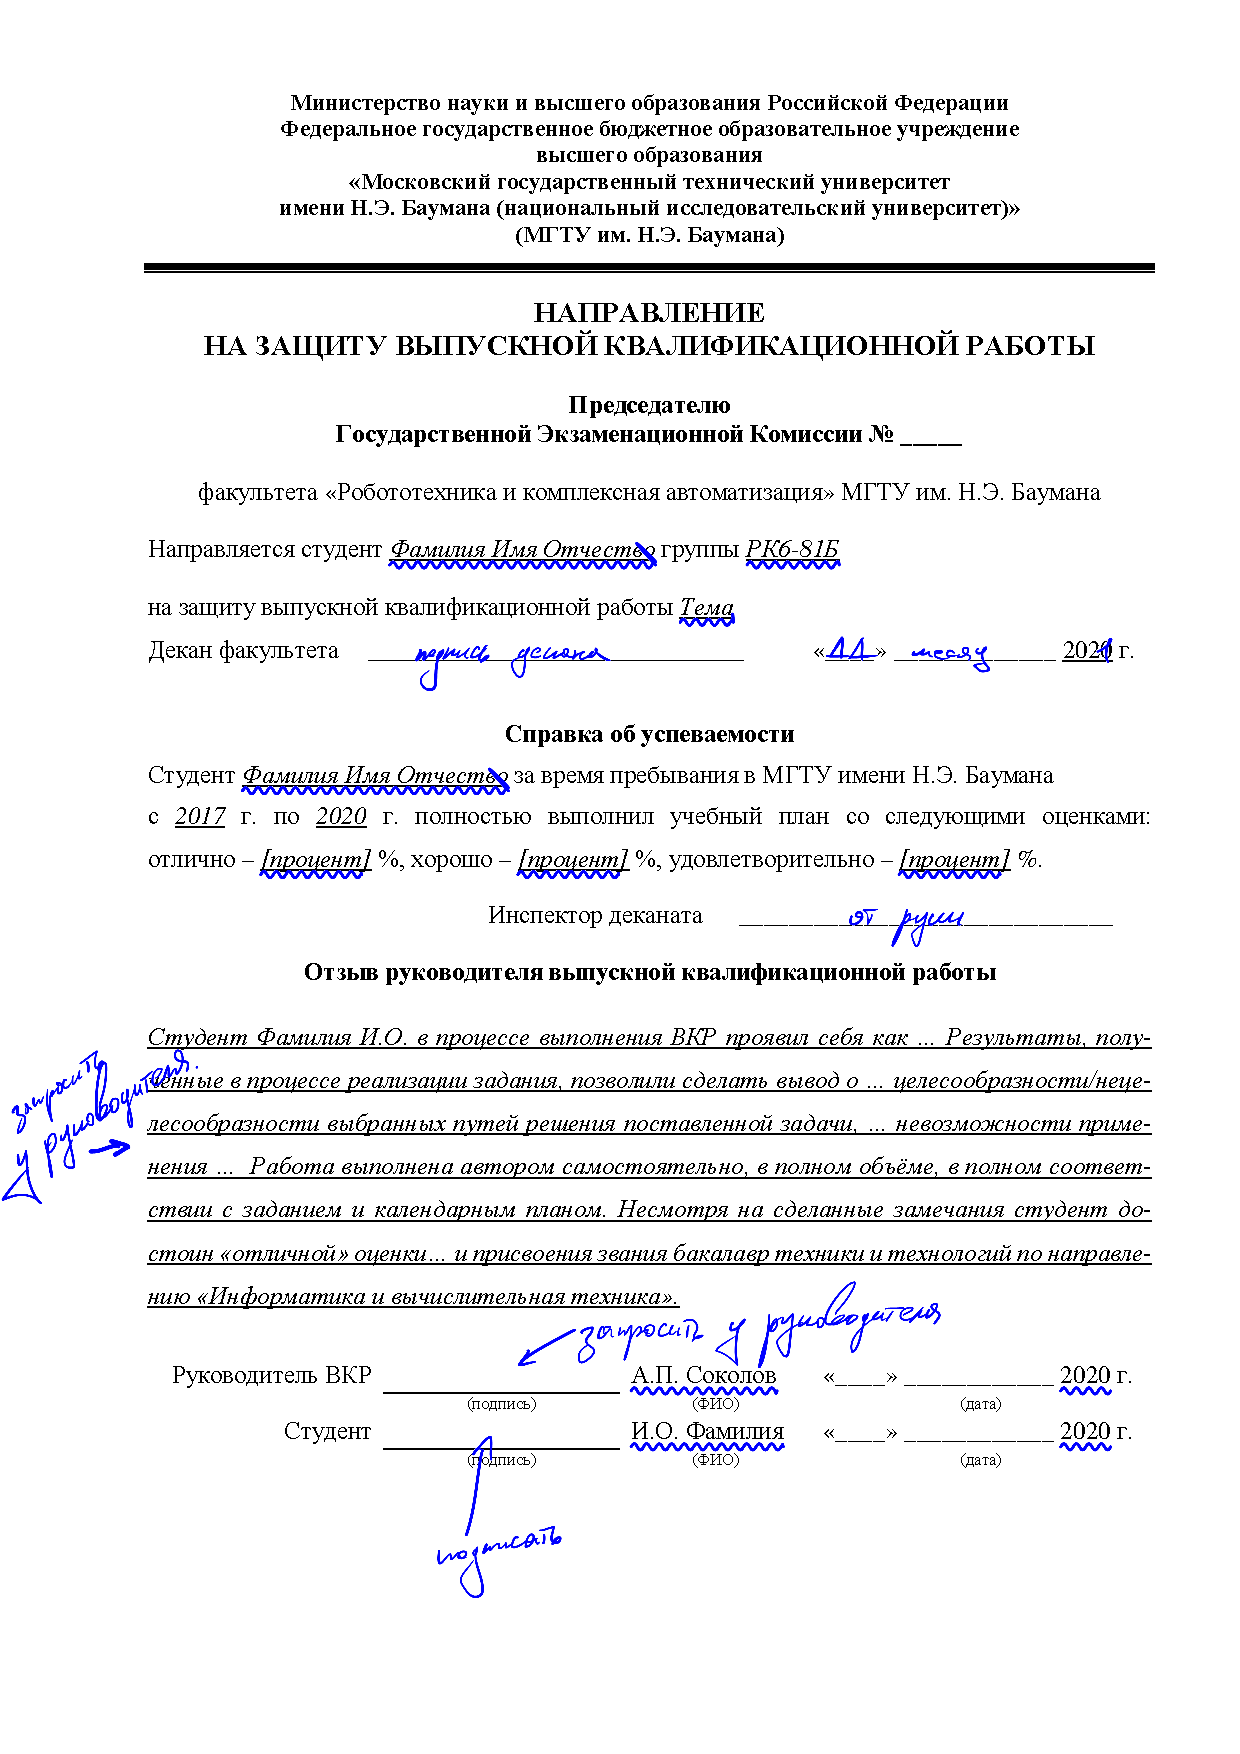
\includepdf{doc-additional/cpxsln_vkr_20YY_ShortTitle_group_SurnameNF_referral_for_defense.pdf}
}
%----------------------------------------------------------------

}
%----------------------------------------------------------
% Реферат
%----------------------------------------------------------
\chapter*{РЕФЕРАТ}
%----------------------------------------------------------
\doctype\xspace: \total{page}~с., \total{ffigure}~рис., \total{ttable}~табл., \total{bibcnt}~источн.%, \textbf{apxchapters} прил.

\vspace{3mm}

%Ключевые слова:
\MakeUppercase{\keywordsru}.

\Preface

\textbf{Тип работы}: \doctype.

\textbf{Тема работы}: \textit{<<\Title>>}.

\textbf{Объект исследования}: \ObjectOfResearch.

\textbf{Основная задача, на решение которой направлена работа}: \MainProblemOfResearch.

\textbf{Цели работы}: \GoalOfResearch

\SubtasksPerformed

% При оформлении согласно ГОСТ 7.32-2001 
%(все освещать следует в этом же порядке - разделы не обязательны)
%объект исследования или разработки
%цель работы
%метод или методологию проведения работы
%результаты работы
%основные конструктивные, технологические и технико-эксплуатационные характеристики
%степень внедрения
%рекомендации по внедрению или итоги внедрения результатов НИР
%область применения
%экономическую эффективновность или значимость
%прогнозные предположения о развитии объекта исследования.


%----------------------------------------------------------
% Сокращения и определения
\newpage
\pagestyle{fancy}
\printglossary[type=abbreviations, title={СОКРАЩЕНИЯ}, nopostdot=false, nonumberlist]
%\thispagestyle{plain}
%\printglossary[type=main, title={ОПРЕДЕЛЕНИЯ}, nopostdot=true]
%----------------------------------------------------------
% Содержание
% Глубина содержания должна быть не более, чем глава (chapter), раздел (section) и подраздел (subsection)
\setcounter{tocdepth}{2}
% Добавление в оглавление сверху Стр.
%\makeatletter
%\addtocontents{toc}{\string\pagestyle{TOC}}
%\addtocontents{toc}{\string\thispagestyle{fancy}}
%\addtocontents{toc}{\hfill Стр.\par}
%\def\ps@TOC{%
    %\def\@oddhead{\hfill \thepage \hfill Стр.} % нечетные хедеры
    %\let\@oddfoot\@empty % нечетные футеры
    %\def\@evenhead{\hfill \thepage \hfill Стр.} % четные хедеры
    %\let\@evenfoot\@empty % четные футеры
%}
%\makeatother
%----------------------------------------------------------
\renewcommand{\contentsname}{\MakeUppercase{Содержание}}
\newpage
%\pagestyle{tocpage}
\tableofcontents
%----------------------------------------------------------
% Введение
{%
\def\thesection{В.\arabic{section}}
\def\thefigure{В.\arabic{figure}}
\def\thetable{В.\arabic{table}}
%----------------------------------------------------------
\chapter*{ВВЕДЕНИЕ}\label{chap.introduction}
\addcontentsline{toc}{chapter}{ВВЕДЕНИЕ}

Применение ориентированных графов очень удобно для построения архитектур процессов обработки данных (как в автоматическом, так и в автоматизированном режимах). Вместе с тем многочисленные возникающие в инженерной практике задачи предполагают проведение повторяющихся в цикле операций. Самым очевидным примером является задача автоматизированного проектирования (АП). Эта задача предполагает, как правило, постановку и решение некоторой обратной задачи, которая в свою очередь, часто, решается путём многократного решения прямых задач. Простым примером являются задачи минимизации некоторого функционала невязки при варьирование параметров объекта проектирования. Каждая итерация сопряжена с решением прямой задачи и сравнением численного результата с требуемым (например, известным из эксперимента). Функционал строят согласно заданному критерию оптимизации. 

Необходимо отметить, что прямые задачи (в различных областях) решаются одними методами, тогда как обратные - другими. Эти процессы могут быть очевидным образом отделены друг от друга за счет применения единого уровня абстракции, обеспечивающего определение интерпретируемых архитектур  алгоритмов, реализующих методы решения как прямой, так и обратной задач. Очевидным способом реализации такого уровня абстракции стало использование ориентированных графов.

Для решения подзадачи визуализации графа необходимо определить, что известно о графе, который будет применяться. Дан ориентированный граф, возможно содержащий циклы и селекторы, так же переходы из узла самого в себя.

Для визуализации графов существует 2 способа визуализации графов:
\begin{enumerate}
\item Силовые алгоритмы визуализации графов - расположить узлы графа так, чтобы все рёбра имели более-менее одинаковую длину, и свести к минимуму число пересечений рёбер путём назначения сил для множества рёбер и узлов основываясь на их относительных положениях, а затем путём использования этих сил либо для моделирования движения рёбер и узлов, либо для минимизации их энергии.

\item Послойное рисование графа - это способ, в котором вершины ориентированного графа рисуются горизонтальными рядами или слоями с рёбрами, преимущественно направленными вниз.

\end{enumerate}

Для размещения графов известны силовые алгоритмы следующих типов\cite{alg-graph}:
\begin{itemize}
\item Force-Directed - вершины представляются как заряженные частицы, которые отталкивают друг друга с помощью физической силы, а рёбра — как упругие струны, которые стягивают смежные вершины
\item Multidimensional scaling - вершины являются силой, а рёбра уже являются пружинами
\item Energy-Based - в этом подходе пытаются описать потенциальную энергию системы и найти положение вершин, которое будет соответствовать минимуму
\end{itemize}

Для решения поставленной задачи не имеет значения к какой категории принадлежит исследуемый алгоритм, поэтому необходимо рассмотреть самые часто упоминаемые, а именно: Fruchterman-Reingold, Алгоритм Идеса, Kamada Kawaii, Force Atlas 2, OpenOrd, Гамма – алгоритм.

Чтобы выбрать нужный для данного случая алгоритм необходимо выделить свойства результирующего графа, по котором будет произведён отбор:
\begin{itemize}
\item Граф является ориентированным
\item Конец графа должен находится в противоположной стороне от начала
\item Максимально допустимый граф является среднего размера
\item В графе могут не иметься циклы
\end{itemize}

В алгоритме Fruchterman-Reingold используется пружинная физическая модель, где вершины определяются как тела системы, а ребра как пружины. Силы могут действовать только на вершины, вес пружин при этом не учитывается. Данные алгоритм не подходит, так как он не предусмотрен для ориентированных графов \cite{alg-fruchterman}.

Алгоритм Kamada Kawaii похож на алгоритм Fruchterman-Reingold, но выбирается вершина, на которую действует максимальная сила, затем остальные вершины фиксируются, энергия системы минимизируется. Данный метод не подходит, так как имеет самую высокое время работы из рассматриваемых - $O(V^3)$ \cite{alg-kamada-kawai}.

Force Atlas 2 представляет граф в виде металлических колец, связанных между собой пружинами. Деформированные пружины приводят систему в движение, она колеблется и в конце концов принимает устойчивое положение. Основная его задача - визуализация графов, в которых имеются подмножества с высокой степенью взаимодействия, таким свойством целевой граф не обладает \cite{alg-force-atlas-2}.

OpenOrd - это алгоритм, специально предназначенный для очень больших сетей, который работает на очень высокой скорости при средней степени точности. Это хороший компромисс для больших сетей, но часто он нежелателен для небольших графов где потеря точности может быть значительной по сравнению с другими подходами к компоновке. Все вершины изначально помещаются в начало координат, а затем проводятся итерации оптимизации. Итерации контролируются через алгоритм имитации отжига. Предназначен для визуализации больших графов \cite{alg-open-ord}, следовательно не подходит для целевого графа, так как он является графом маленького или среднего размера.

Гамма - алгоритм основная идея которого заключается в том, что выделяются сегменты, затем в минимальном выделяется цепь, которая укладывается в любую грань, вмещающую данный сегмент \cite{alg-gamma}. Не подходит, так как в целевом графе может не оказаться циклов.

Алгоритм Идеса (Magnetic-Spring Algorithm) рёбра назначаются магнитной пружиной, и затем при воздействии магнитных полей вершины перемешаются \cite{alg-eades}. Лучше всего для целевого графа.

Для любого из способа существуют графы, при визуализации которых может появиться неудовлетворительный вид. Однако в следствии того, что послойное рисование графа представляет более привычный вид ориентированного графа был выбран алгоритм из этого типа. Исходя из этого для решения задачи визуализации графа, бы выбран алгоритм dot.

Алгоритм состоит из 4 этапов - \textsf{rank}, \textsf{ordering}, \textsf{position}, \textsf{make-splines}.

В первом этапе каждому узлу необходимо определить ранг для всех узлов. Определение ранга происходит в результате "естественного" обхода. Наличие циклов не позволяет корректно пройтись по графу, поэтому необходимо разорвать циклы. Разрываются они через использование алгоритма DFS, после для каждого узла уже рассчитывается ранг.

После присвоения ранга, ребра между узлами, которые отличаются на более чем на один ранг заменяются цепочками ребер единичной длины между временными или «виртуальными» узлами. Виртуальные узлы размещаются на промежуточных рангах, превращая исходный граф в граф, ребра которого соединяют только узлы на соседних рангах. Порядок вершин в рангах определяет количество пересечений ребер, поэтому хорошим порядком является тот, который имеет наименьшим количеством пересечений. 

Третий проход является этап корректировки. Он нужен для того, чтобы избежать плохих расположений узлов графа. Координаты X и Y вычисляются в два отдельных шага. На первом этапе всем узлам (включая виртуальные узлы) присваиваются координаты X в соответствии с уже определенным порядком внутри рангов. На втором этапе назначаются координаты Y, присваивая одинаковое значение узлам одного ранга. 

После этого в последнем этапе определяются и рисуются ребра, которые будут представлены в виде сплайна. Алгоритм попытается найти самую гладкую кривую между двумя точками, которая избегает «препятствий» в виде других узлов или сплайнов. Затем разделит алгоритм маршрутизации сплайнов на верхнюю половину и нижнюю половину. Верхняя половина вычисляет многоугольную область макета, где может быть нарисован сплайн. Она вызывает нижнюю половину для вычисления наилучшего сплайна в области\cite{alg-dot}.

Для решения задачи обхода графа из-за специфичности задачи было принято решение о создании собственного алгоритма. Особенностями больше всего влияющие на решение создания алгоритма являются - наличие селекторов, проход не всегда по всему графу.

Далее при описании алгоритма используется терминология, введённая в работах \cite{SokPersh2019PCS, SokGolub2021GBSEBL}.

Рассмотрим некоторый узел $S_i$ орграфа $G$, из которого выходит множество рёбер $E_i=\{e_{ij}\}_1^n$, $n>0$. Для построения алгоритма обхода необходимо определить правила перехода от узла $S_{i}$ к другим узлам.
\begin{enumerate}
  \item Если $n=1$, то переход безусловный, т.е. предполагает вызов связанной с $e_{ij}$ функции перехода $F_{ij}$, где $j$ соответствует номеру следующего узла $S_j$.
  \item Если $n>1$, то переход следует осуществлять по всем рёбрам, которые определяются с помощью функции-селектора $h_i$ (организует ветвление, рис.~\ref{rndhpcedt.20230201.1}), сопоставленной с узлом $S_i$, результат выполнения которой определяет подмножество $\hat{E}_i=\{a_{ik}\colon {a_{ik}\in E_i}, {\pr_k(h_i(D_i))=1}, {D_i \filledemptyspoon S_i}\}$, где $S_i$ -- состояние данных \gls{ccm}, сопоставленное с одноимённым узлом $S_{i}$, $D_i$ -- данные в состоянии $S_i$, $\pr_{i}(r)$ -- операция проекции объекта $r$ на $i$-ю координату. Порядок выбора рёбер из $\hat{E}_i$ для осуществления перехода не важен.
\end{enumerate}

\begin{remark}
Реализация $\hat{E}_i$ для каждого $i$ возможна путём формирования структуры данных стек. Заполнение соответствующего стека элементами может быть осуществлено в произвольном порядке\footnote{Должны быть выполнены все функции перехода $F_{ij}$, связанные с соответствующими рёбрами, в произвольном порядке (возможно в многопоточном режиме).}.
\end{remark}

Для реализации требуемого алгоритма необходимо: сделать класс дуги и в класс узла добавить поля, которые определяют необходимое число для перехода через данный узел и количество дуг, которые уже пришли в узел. Класс дуги содержит два поля: начальный узел и конечный узел.

Рассмотрим работу алгоритма на примере орграфа, представленного на рисунке~\ref{fig:graph}. Начальная вершина называется \textsf{Start}, а конечная \textsf{End}. Селекторы в данном примере отсутствуют.

Рассмотрим алгоритм перехода из узла \textsf{Start}. Так как из узла \textsf{Start} выходит два ребра, то выбираем случайное из них (например, ребро \textsf{Start$\rightarrow$A}), совершаем соответствующий переход\footnote{Выполняем соответствующую функцию перехода при \flqq боевом \frqq режиме обхода.}, тогда как оставшееся ребро \textsf{Start$\rightarrow$B} заносится в стек. После перехода в \textsf{A}.  Затем из-за того, что всего доступна только одна вершина, переход происходит в вершину \textsf{C}.

Далее происходит ситуация, что из вершины опять выходит два ребра. Аналогичным образом для перехода выбираем, например, ребро \textsf{C$\rightarrow$E}, тогда в стек заносится ребро \textsf{C$\rightarrow$F}. После выполнения перехода в вершину \textsf{E} ещё раз необходимо выполнение таких же действий. Допустим переход осуществляется по ребру \textsf{E$\rightarrow$D}, а \textsf{E$\rightarrow$G} заносится в стек. На текущий момент в стеке находится три ребра - \textsf{Start$\rightarrow$B}, \textsf{C$\rightarrow$F}, \textsf{E$\rightarrow$G}.

После выполнения перехода в вершину \textsf{D} оказывается, что она требует для продолжения выполнение перехода ещё по ребру \textsf{B$\rightarrow$D}. Следовательно, из стека достаётся ребро - \textsf{E$\rightarrow$G} и осуществляется переход по данному ребру. Далее, при попытке переход через вершину \textsf{G} получается, что необходимо выполнения ребра \textsf{D$\rightarrow$G}, достаётся следующее ребро из стека. Далее выполняется переход по ребру \textsf{C$\rightarrow$F}. Аналогично переход по ребру \textsf{F$\rightarrow$H}. Далее вершина \textsf{H} для продолжения обхода требует переход по \textsf{G$\rightarrow$H}. Из-за этого берется ребро из стека и выполняется переход по нему.

Затем, после перехода по ребру \textsf{B$\rightarrow$D}, в вершине \textsf{D} проверяется разрешается ли переход далее. Так как все нужные для продолжения обхода ребра уже пройдены, то переход разрешается. Далее из этой вершины по ребру \textsf{D$\rightarrow$G} осуществляется переход. В вершине \textsf{G} повторяется аналогичная ситуация, поэтому осуществляется переход по ребру \textsf{G$\rightarrow$H}. Далее по такому же правилу алгоритм доходит до вершины \textsf{End}, чем заканчивает обход.

В разработанном А.П.~Соколовым и А.Ю.~Першиным графоориентированном программном каркасе, для описания графовых моделей был разработан формат aDOT, который является расширением формата описания графов DOT.

Для визуализации графов, описанных с использованием формата DOT, используются специальные программы визуализации. Формат aDOT расширяет формат DOT с помощью дополнительных атрибутов и определений, которые описывают функции-предикаты, функции-обработчики и функции-перехода в целом. Из этого вытекает, что для построения графовых моделей с использованием формата aDOT необходим графический редактор.
}
%----------------------------------------------------------
\mainmatter %% это включает нумерацию глав и секций в документе ниже
%----------------------------------------------------------
%=============================================================
%----------------------------------------------------------
\chapter{Постановка задачи}
%----------------------------------------------------------
\section{Концептуальная постановка задачи}
Дано: ориентированный граф $G$ (орграф), возможно, содержащий циклы, определённый множествами узлов $\{S_i\}_1^m$ и рёбер $\{e_{ij}\colon i\in[1\ldotp\ldotp M], j\in[1\ldotp\ldotp N]\}$, где $M,N$ -- некоторые целые числа.

Разрабатываемый графический редактор должен:
\begin{enumerate}
\item  Предоставлять возможность создавать ориентированный граф с нуля (добавление/удаление ребра/узла)
\item Предоставлять возможность обхода графа
\item Предоставлять возможность экспортировать созданный граф в формат aDOT
\item Предоставлять возможность загрузить граф из формата aDOT
\end{enumerate}

Так же должен удовлетворять следующим требованиям:
\begin{itemize}
\item Иметь возможность экспорта программного кода на языке программирования Python
\item Являться плагином для comwpc
\end{itemize}

В конечном итоге выполнения должен осуществляться визуализаци и обход с выполнением python-кода по всему графу, который, возможно, задан в файле формата aDOT. 
%----------------------------------------------------------
%%----------------------------------------------------------
\chapter{Вычислительный метод}\label{chap2_comp_method}
%----------------------------------------------------------
%\section{Концептуальная постановка задачи}

В разделе следует представить описание применяемого (планируемого к применению) вычислительного метода. Метод следует описывать с использованием математически строгих формулировок, не допускающих неоднозначности прочтения.

Обязательность представления: раздел представляется в зависимости от поставленной задачи.
Объём: около 5 страниц.

%----------------------------------------------------------


%----------------------------------------------------------
%----------------------------------------------------------
\chapter{Программная реализация}\label{chap3_soft_architecture}
%----------------------------------------------------------
\section{Архитектура}

Для разработки было принято решение использовать язык программирования Python3.10 и библиотеку networkx для работу с графом.

В реализации программы должны быть реализованы четыре главных сценария действия: Открыть из файла, создание графа, сохранение в файлы, найти цикл. Так же необходимо создать простую базу данных для хранения графов для каждого пользователя. Общий вид схемы модулей представлен на рисунке \ref{fig:module}. В программе должно быть реализована 2 класса - Graph (класс графа) и Node (класс вершина). 

В классе узла должны иметься следующий поля: словарь с ключом в виде следующих узлов и код при переходе к следующему узлу, являющимся значением являющейся строкой; название для узла.

Краткое описание модулей и их взаимодействия:
\begin{itemize}
\item Открыть из файла - модуль , для этого необходимо реализовать алгоритм укладки графа и парсер для преобразования из файла типа aDot в массив объектов класса узла.
\item Создать новый граф - модуль ответственный за добавление/удаление частей графа с помощью ручного ввода.
\item Сохранение в файл - модуль ответственный за сохранения графа в файл типа aDot, для этого необходимо реализовать парсер для преобразования в нужный форма из массива объектов класса узла.
\item Найти цикл - модуль ответственный за нахождение цикла в графе, для этого необходимо реализовать алгоритм поиска цикла в графе.
\end{itemize}

В классе графа в полях должно иметься массив класса узлов, в методах должны быть реализованы:
\begin{itemize}
\item make\_graph(name) - метод, которые преобразует массив в объекте класса в переменную, которую можно сохранить в виде изображения с выбранным расширением.
\item read\_from\_aDot(name) - метод, читающей из файла с названием name (тип string) данные, затем сохраняет их в поле для узлов. 
\item search\_cicles() - метод, который находит циклы в графе, возвращает все циклы в виде строки формата "a-b-c[перенос строки]b-d-e[перенос строки]".
\item add\_eage(e1, e2) - метод, добавляющий ребро между двумя узлами из e1 (тип класса узла) в e2 (тип класса узла)
\item delete\_eage(e1, e2) - метод, удаляющий ребро между двумя узлами из e1 (тип класса узла) в e2 (тип класса узла)
\item add\_node(node) - метод, добавляет узел node
\item delete\_node(node) - метод, удаляющий узел node
\item save\_into\_aDot(name) - метод, сохраняет граф в файл с названием name (тип string)
\end{itemize}

В базе данных необходимо иметь одну таблицу с двумя полями: пользователь и его граф.

%----------------------------------------------------------
%----------------------------------------------------------
\chapter{Тестирование и отладка}\label{chap4_soft_testing}
%----------------------------------------------------------
\section{Экспорт графа в aDOT файл}
Для тестировании основная функционал и экспорта в файл с помощью доступных инструментов сделаем граф показанный на рисунке(\ref{g1}).

В результате должен получиться файл с описание графовой модели в формате aDOT представленным на листинге (\ref{l1}).
\begin{lstlisting}[label=l1, caption={\textit{Полученное описание графовой модели в формате aDOT}}]
digraph TEST
{
// Parallelism
s1 [parallelism=threading]
s2 [parallelism=threading]
// Function
f1 [module=f1_module, entry_func=f1_function]
// Predicates
p1 [module=p1_module, entry_func=p1_function]
// Transition
edge_1 [predicate=p1, function=f1]
// Graph model
__BEGIN__ -> s1
s1 => s2 [morphism=edge_1]
s1 => s3 [morphism=edge_1]
s2 => s4 [morphism=edge_1]
s2 => s5 [morphism=edge_1]
s3 -> s7 [morphism=edge_1]
s4 -> s6 [morphism=edge_1]
s5 -> s6 [morphism=edge_1]
s6 -> s9 [morphism=edge_1]
s7 -> s8 [morphism=edge_1]
s8 -> s9 [morphism=edge_1]
s9 -> __END__
}
\end{lstlisting}

\section{Импорт из aDOT файла}
Тестирование производится путём импорта файла из предыдущего пункта. В случае успешного выполнения получится граф представленный на рисунке (\ref{g2}). Стоит отметить, что внешний вид изменится за счёт применения алгоритма визуализации.

\section{Тестирование циклов в графе}
В описание графовой модели на предыдущем шаге добавим несколько циклов и обратных ребер. Получим следующее описание графовой модели представленное на листинге (\ref{l2}).
\begin{lstlisting}[label=l2, caption={\textit{ Пример описание графовой модели в формате aDOT включающей циклы}}]
digraph TEST
{
// Parallelism
s7 [parallelism=threading]
s11 [parallelism=threading]
s2 [parallelism=threading]
s10 [parallelism=threading]
s1 [parallelism=threading]
// Function
f1 [module=f1_module, entry_func=f1_function]
// Predicates
p1 [module=p1_module, entry_func=p1_function]
// Transition
edge_1 [predicate=p1, function=f1]
// Graph model
__BEGIN__ -> s1
s4 -> s6 [morphism=edge_1]
s5 -> s6 [morphism=edge_1]
s7 => s6 [morphism=edge_1]
s7 => s1 [morphism=edge_1]
s11 => s8 [morphism=edge_1]
s11 => s2 [morphism=edge_1]
s12 -> s8 [morphism=edge_1]
s2 => s4 [morphism=edge_1]
s2 => s5 [morphism=edge_1]
s2 => s7 [morphism=edge_1]
s10 => s11 [morphism=edge_1]
s10 => s12 [morphism=edge_1]
s1 => s2 [morphism=edge_1]
s1 => s10 [morphism=edge_1]
s6 -> s9 [morphism=edge_1]
s8 -> s9 [morphism=edge_1]
s9 -> s6 [morphism=edge_1]
s9 -> __END__
}
\end{lstlisting}

В случае успешной загрузки графа получим модель графа, представленной на рисунке (\ref{g3}).
%----------------------------------------------------------
%%----------------------------------------------------------
\chapter{Вычислительный эксперимент}\label{chap5_comp_experiment}
%----------------------------------------------------------
\section{...}

В разделе следует представить описания каждого вычислительного эксперимента, включая указание особенностей их проведения, используемые программные средства, используемые исходные данные, принципы запуска с указанием ожидаемого и полученного результата.

Обязательно представление графических результатов в форме графиков, поверхностей.

Обязательность представления: раздел представляется в зависимости от постановки задачи.

Объём: объём не ограничен, но, как правило, не должен быть меньше 5-6 страниц.

%----------------------------------------------------------
%\section{...}

%----------------------------------------------------------


%----------------------------------------------------------
%----------------------------------------------------------
\chapter{Анализ результатов}\label{chap6_results_analysis}
%----------------------------------------------------------

По результатам тестирования можно сделать вывод о работоспособности программы по части базовых функций. Предоставленные графы успешно обходятся. Формирование из aDot представляет собой удобочитаемый граф. Запись в aDot файл происходит в соответствии требованиям для этого формата.

Технически предусмотрена возможность добавления обработки новых атрибутов вершин и дуг графа в файле формате aDot. Потенциально можно добавить несколько алгоритмов визуализации или обхода графов.

На текущей стадии разработки программа не является web-приложение, что планируется исправится в дальнейшем. Так же несмотря на присутствие "заглушек" для исполнения Python-кода, сам функционал его исполнения и добавления, пока не создан.
%----------------------------------------------------------
%\section{...}

%----------------------------------------------------------


%=============================================================

%----------------------------------------------------------
\backmatter %% Здесь заканчивается нумерованная часть документа и начинаются Заключение и Список использованных источников
%----------------------------------------------------------
%----------------------------------------------------------
\chapter*{ЗАКЛЮЧЕНИЕ}\label{chap_conclusion}
\addcontentsline{toc}{chapter}{ЗАКЛЮЧЕНИЕ}
%----------------------------------------------------------

Была проведена работа по изучению алгоритмов визуализации графов, выделены основные их виды. После просмотра на практике были выделены недостатки и особенности каждого из них, после чего принято решение об использовании алгоритма dot.

Разобраны виды обхода графов, однако из-за специфичности задачи было принято решение о создании собственного алгоритма. Особенностями больше всего влияющие на решение создания алгоритма являются - наличие селекторов, проход не всегда по всему графу.

По результатам тестирования выявлено, что программы выполняет большинство требуемых базовых функций.

Программа сделана с учётом на будущее дополнения каких-либо частей, а именно:
\begin{itemize}
\item Добавления новых атрибутов вершин и дуг графа в файле формате aDot.
\item Использование множества алгоритмов визуализации графов с возможностью выбора определённого.
\item Добавление нескольких алгоритмов обхода графов и возможность выбора какой из них будет использоваться для данного графа.
\end{itemize}
%----------------------------------------------------------

%----------------------------------------------------------
% Список литературы
\bibliographystyle{utf8gost705u}
\addcontentsline{toc}{chapter}{Литература}
\bibliography{bibliography}
%----------------------------------------------------------
\subsubsection*{Выходные данные}
%----------------------------------------------------------
\textit{\DocOutReference}
%----------------------------------------------------------
% Атрибуты задачи
\docattributes{}{}{}{}{студент группы \group, \Author}{\Year, \Semestr}
%----------------------------------------------------------
% Акт об отсутствии заимствования (включается только для ВКР, для НИРС и КП не нужно)
% Вставится только при сборке ВКР
\myconditionaltext{\doctypesid}{vkr}{%
		%----------------------------------------------------------------
% В этот документ следует вставить акт об отсутствии заимствования
% Для КП, НИРС этот документ не включается.
% Предварительно документ следует подготовить в MS Word, подписать, преобразовать в PDF и далее разместить в нужном каталоге
\newpage
{\catcode`\_=11
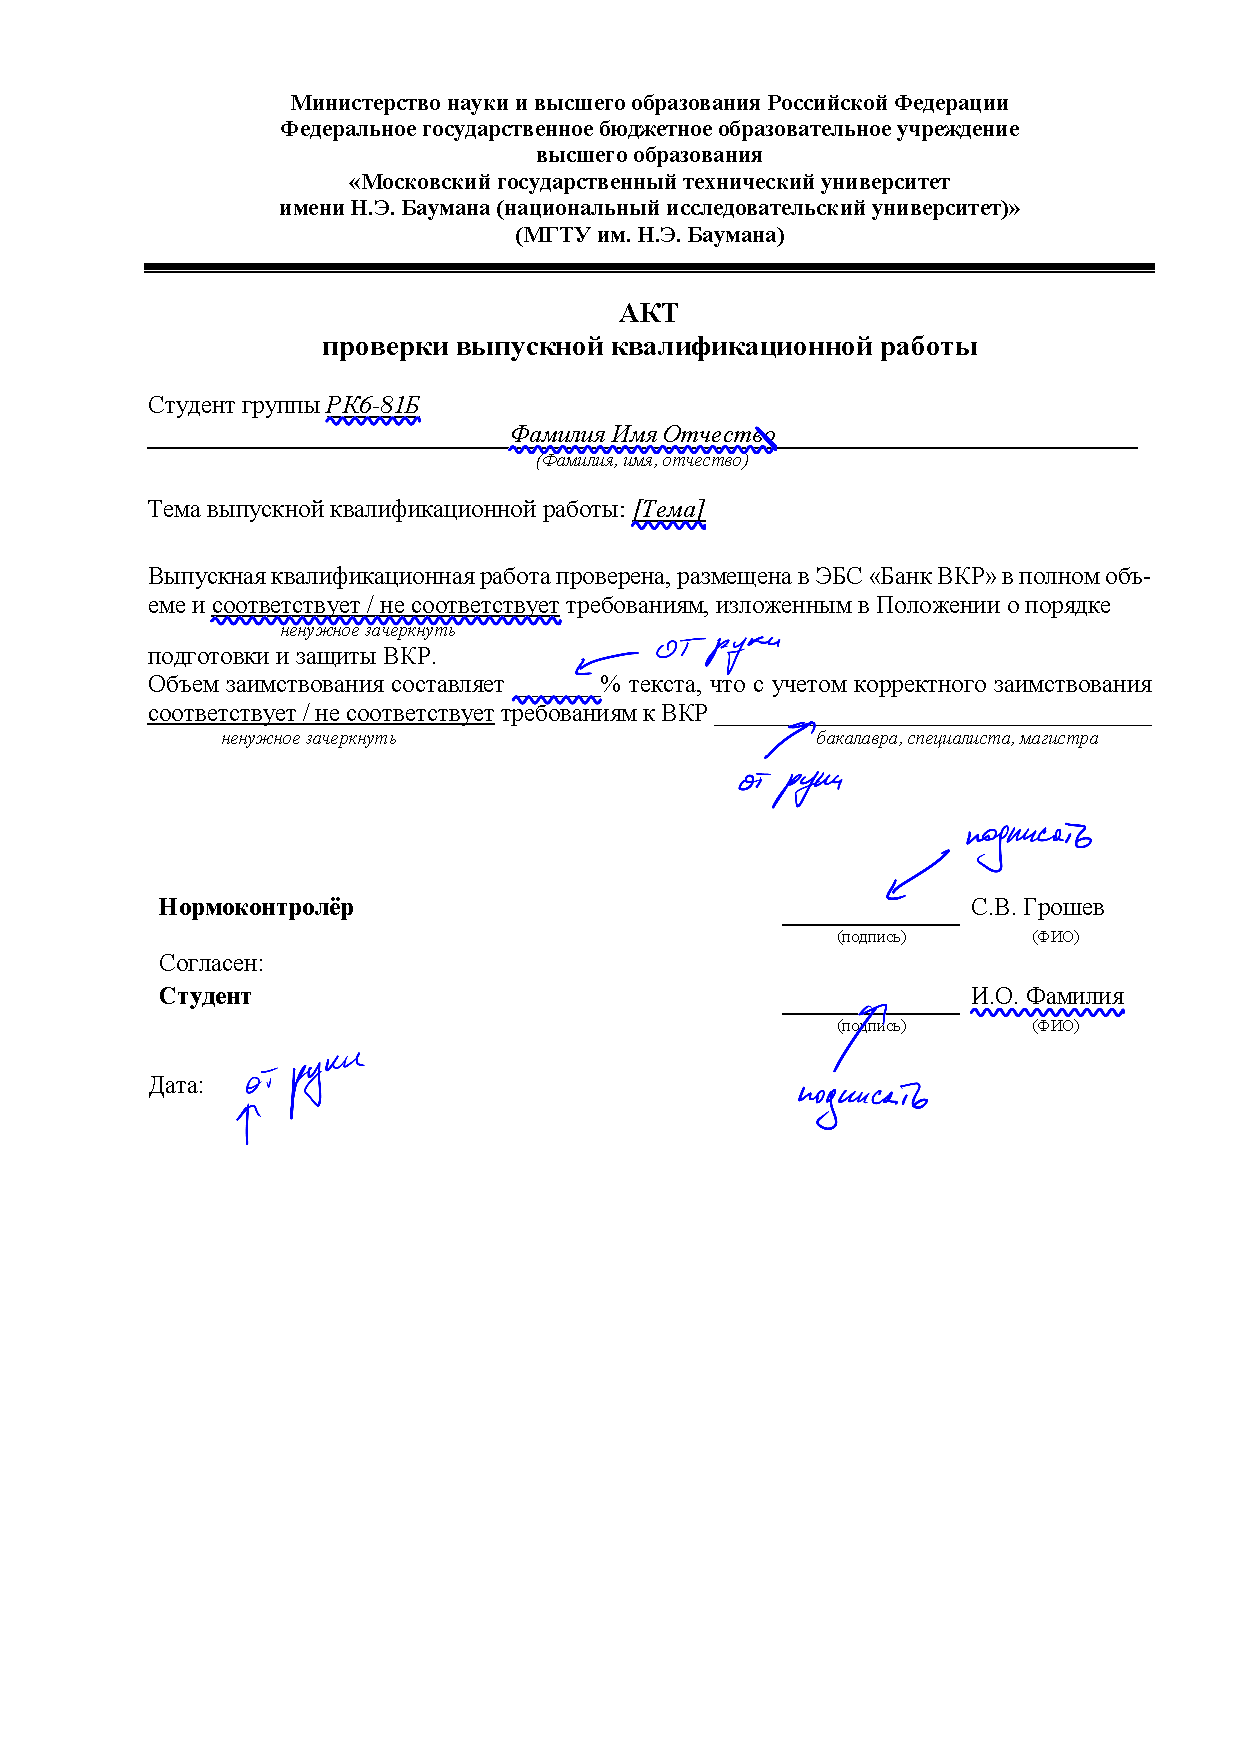
\includepdf{doc-additional/cpxsln_vkr_20YY_ShortTitle_group_SurnameNF_plagiarism.pdf}
}
%----------------------------------------------------------------

}
%----------------------------------------------------------
%приложения
%
% листы A1
% Акт об отсутствии заимствований
% Рецензии
%

\appendix

% команды далее необходимы для того, чтобы нумерация элементов текста в приложениях была корректной.
\renewcommand{\theequation}{\thechapter.\arabic{equation}}
\renewcommand{\thefigure}{\thechapter.\arabic{figure}}
\renewcommand{\thetable}{\thechapter.\arabic{table}}
% -------
\renewcommand{\appendixname}{ПРИЛОЖЕНИЯ}
\def\chaptername{ПРИЛОЖЕНИЕ}
\def\thechapter{\Asbuk{chapter}\unskip}
\renewcommand{\thesection}{\thechapter.\arabic{section}\unskip}
%%%%%%%%%%%%%%%%%%%%%%%%%%%%%%%%%%%%%%%%%%%%%%%%%%%%%%%%%%%%%%%%%%%%%%%%
\addcontentsline{toc}{chapter}{ПРИЛОЖЕНИЯ}
%%%%%%%%%%%%%%%%%%%%%%%%%%%%%%%%%%%%%%%%%%%%%%%%%%%%%%%%%%%%%%%%%%%%%%%%
% ПРИЛОЖЕНИЕ
\fancyhead[C]{\thepage \\ \textbf{\leftmark}}
\fancyfoot[C]{}
%----------------------------------------------------------------
\includepdfset{turn=true,scale=0.85,linktodoc=true,pages=-,pagecommand={\pagestyle{fancy}}}
%----------------------------------------------------------------
\chapter{}\label{apx_a1}

\begin{figure}[!ht]
	\centering
	\def\udoffset{10mm}
	\tikzstyle{ar} = [->, >={Stealth[length=8pt]}]
	\tikzstyle{tx} = [midway,sloped,anchor=center, above]
	\begin{tikzpicture}[node distance=2.8cm, scale=1.4]
		\node[state] (S) [xshift=-10mm] {$S_i, h_i$};
		\node[state] (S0) [left of=S] {$\cdots$};
		\node (Sm1) [left of=S0] {$\cdots$};
		\draw [ar] (Sm1) -- (S0);
		\draw [ar] (S0) -- (S);
		\node[state] (S1) [above right of=S, xshift=5mm] {$S_1$};
		\node[state] (S2) [right of=S, xshift=5mm] {$S_2$};
		\node (S11) [right of=S1, xshift=-5mm] {$\cdots$};
		\node (S12) [right of=S2, xshift=-5mm] {$\cdots$};
		\draw [dashed,ar] (S) -- node [tx] {\small $e_{i1}, b_1=1$} (S1);
		\draw [ar] (S1) -- (S11);
		\draw [dashed,ar] (S) -- node [tx] {\small $e_{i2}, b_2=0$} (S2);
		\draw [ar] (S2) -- (S12);
		\draw [dashed,ar] (S) .. controls +(north:1.25*\udoffset) and +(north:1.25*\udoffset) .. node [tx] {\small $e_{i3}, b_3=0$} (S0);
	\end{tikzpicture}
	\caption{Организация ветвления с помощью функции-селектора $h_i$ из состояния $S_i$, где $\forall D_i\filledemptyspoon S_i\rightrightarrows\{S_j\}_{j=1}^{n}$ и $h_i(D_i)=\mbf{b}=(b_1,b_2,b_3,\ldots,b_n)=(1,0,0,\ldots)$. Очевидно, что для представленной иллюстрации $\hat{E}_i=\{e_{i1}\}$ и переход по ветвям, для которых $b_i=0$, запрещён}
	\label{rndhpcedt.20230201.1}
\end{figure}

\chapter{}\label{apx_a2}
\begin{figure}[h]
    \centering
    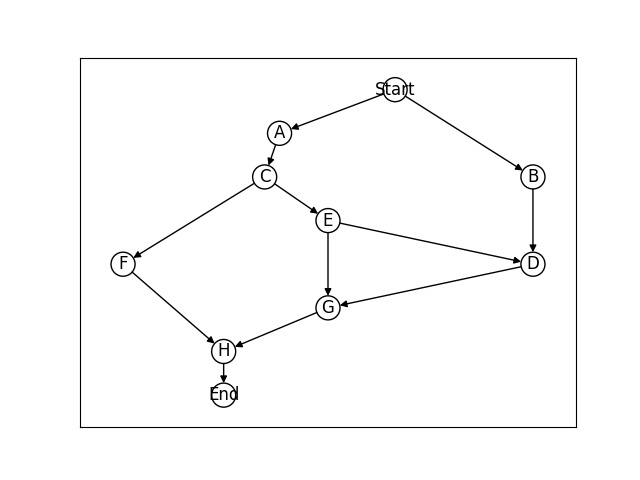
\includegraphics[width=0.55\linewidth]{images/graph.jpg}
    \caption{Пример орграфа без циклов}
    \label{fig:graph}
\end{figure}

\chapter{}\label{apx_a3}
\begin{figure}[h]
    \centering
    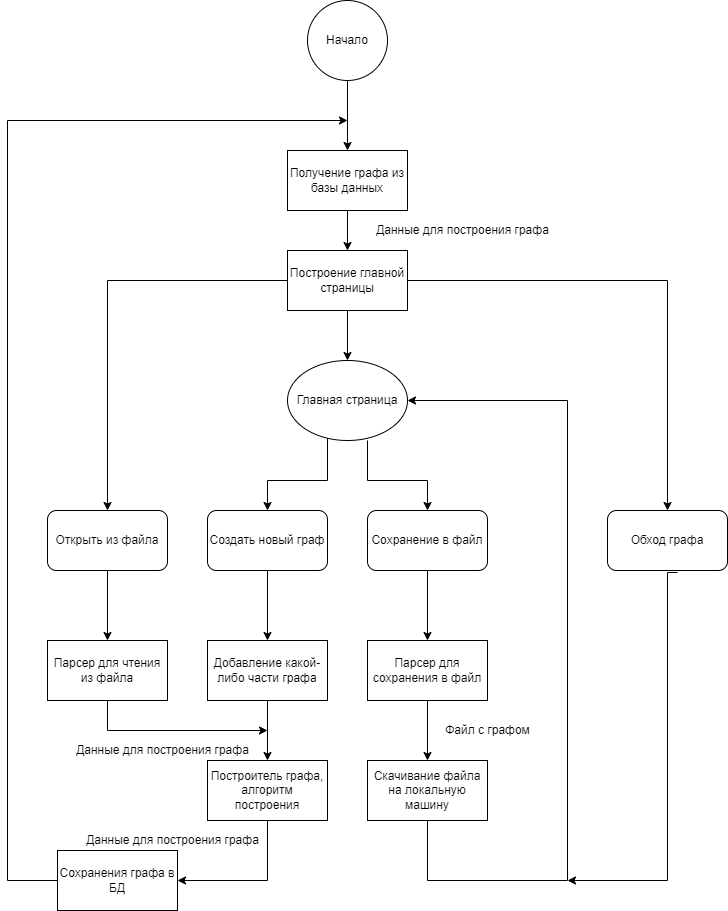
\includegraphics[width=0.7\linewidth]{images/module.png}
    \caption{Схема модулей программы}
    \label{fig:module}
\end{figure} 

\chapter{}\label{apx_a4}
\begin{figure}[!h]
\centerline{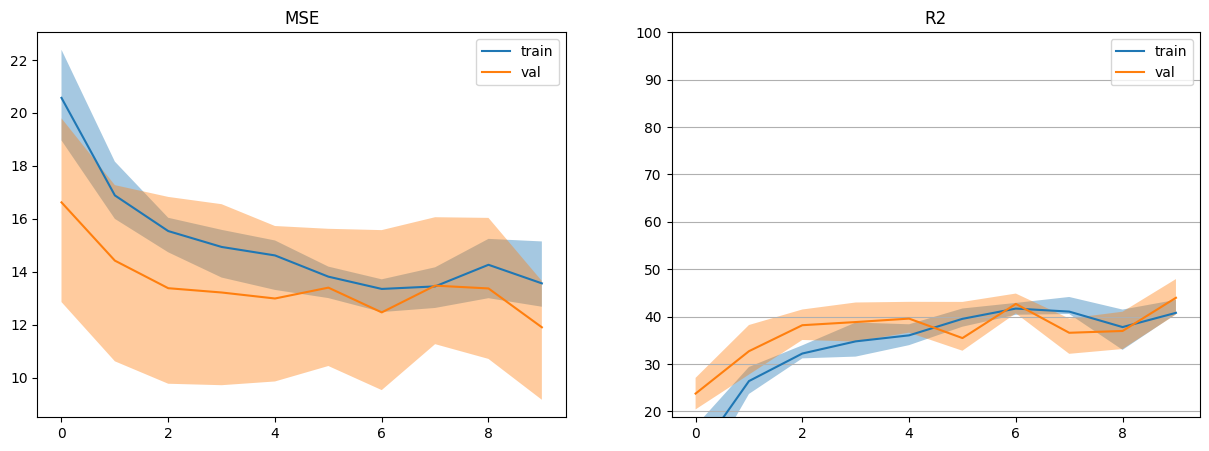
\includegraphics[scale=0.5]{images/1.png}}
\caption{Ориентированный граф созданный с нуля в редакторе}
\label{g1}
\end{figure}

\chapter{}\label{apx_a5}
\begin{figure}[!h]
\centerline{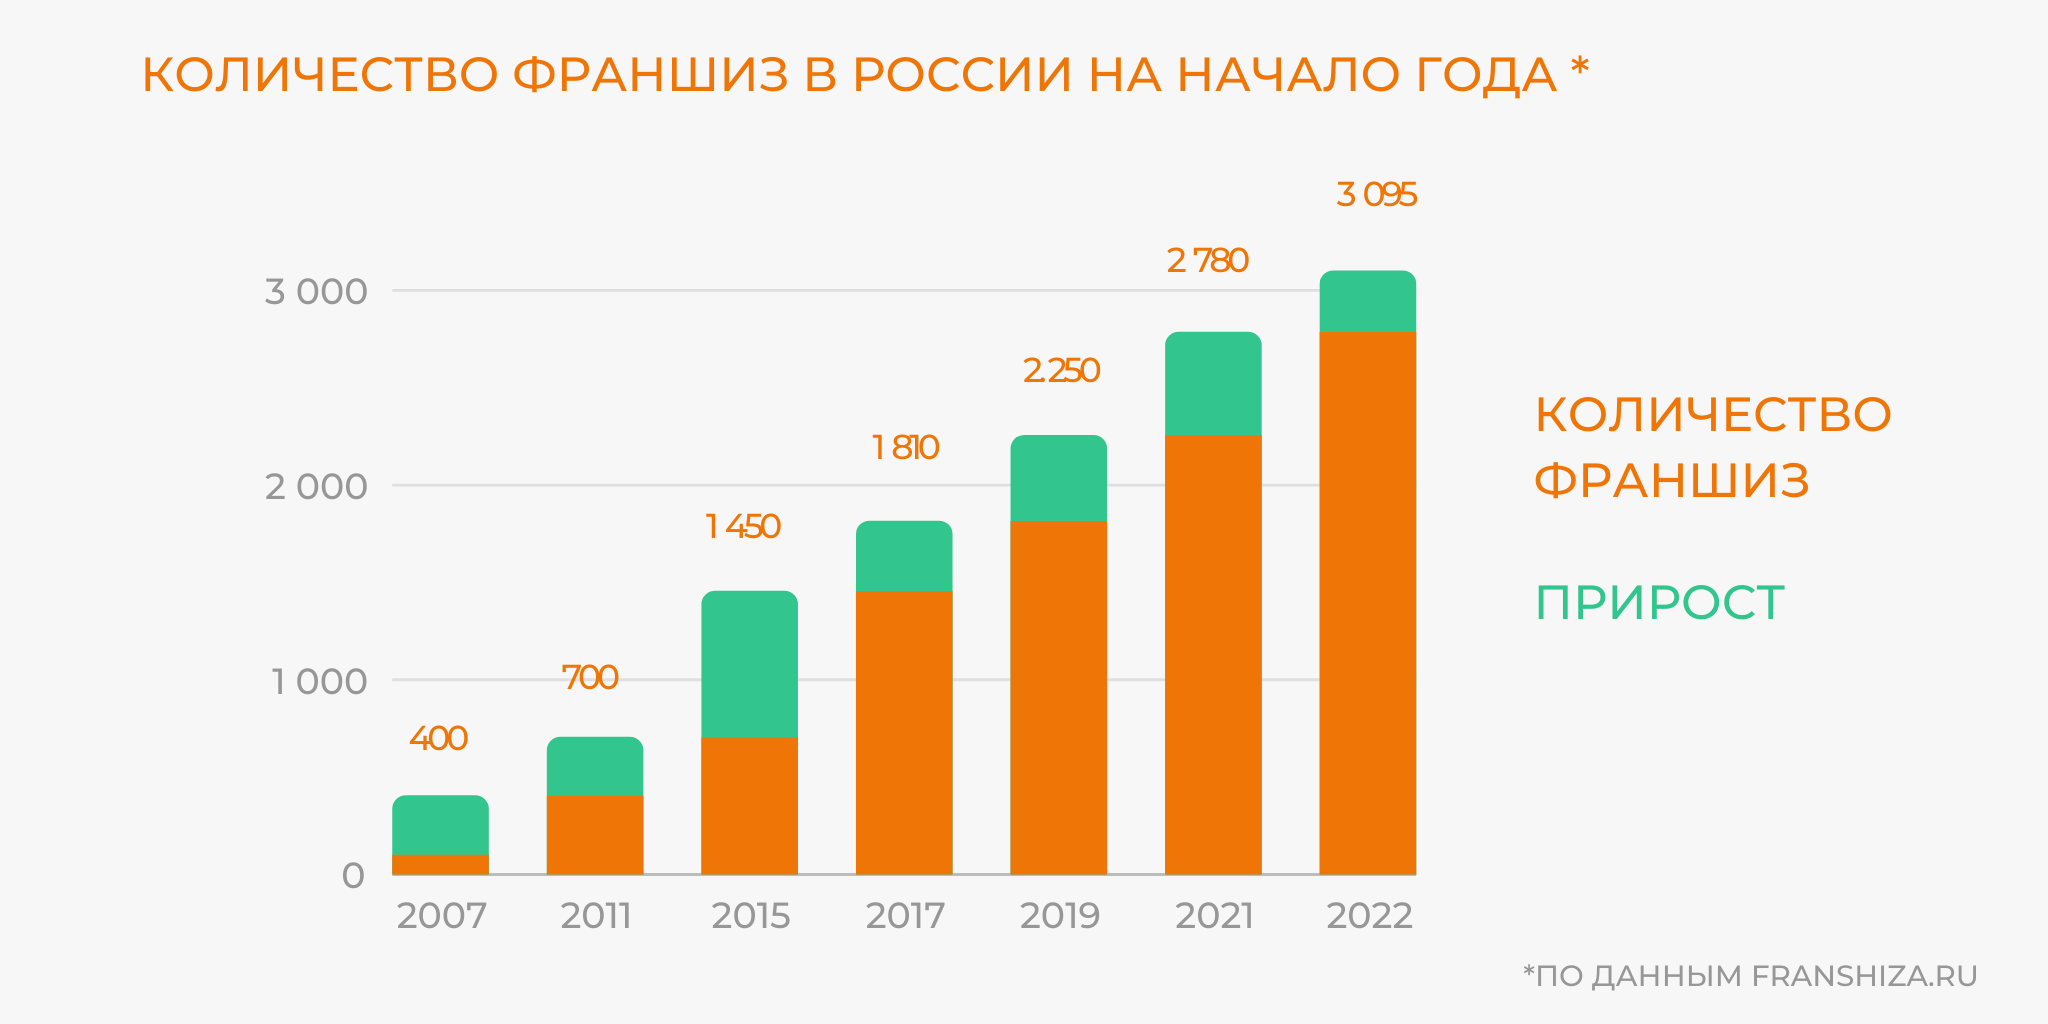
\includegraphics[scale=0.5]{images/2.png}}
\caption{Загруженный в формате aDOT граф}
\label{g2}
\end{figure}

\chapter{}\label{apx_a6}
\begin{figure}[!h]
\centerline{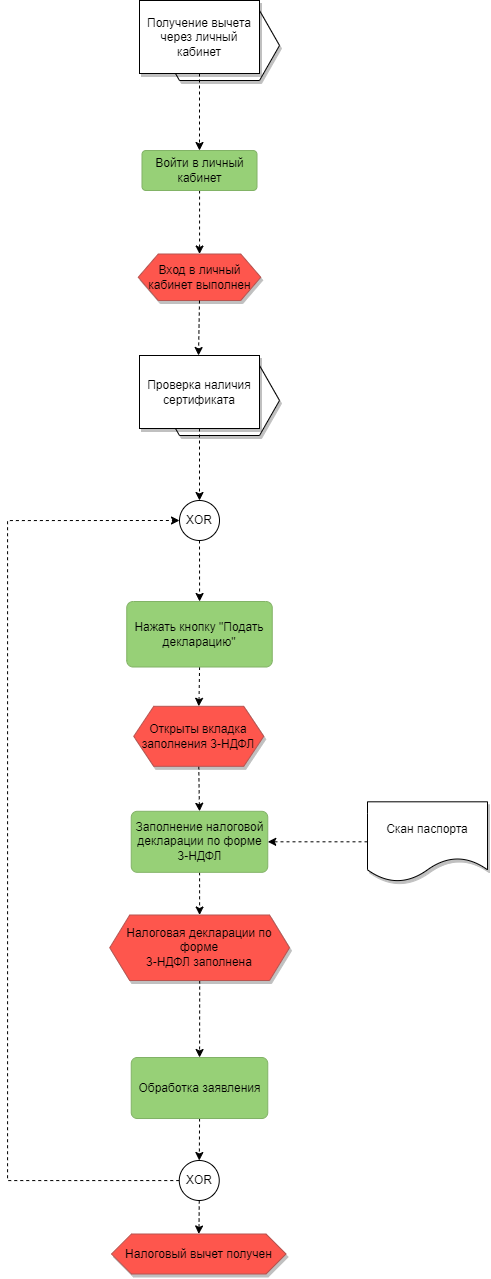
\includegraphics[scale=0.5]{images/4.png}}
\caption{Загруженный в формате aDOT граф}
\label{g3}
\end{figure}
%{\catcode`\_=11
%\newpage
%\includepdf[pagecommand=\label{appx_A1_list1},pages=-]{appendices/appx_A1_list1.pdf}
%}
%
%%{\catcode`\_=11
%%\newpage
%%\includepdf[pagecommand=\label{appx_A1_list1},pages=-]{appendices/appx_A1_list1.pdf}
%%}
%%----------------------------------------------------------------
%\chapter{Акты и рецензии}\label{apx_acts_reviews}
%
%{\catcode`\_=11
%\newpage
%\includepdf[pagecommand=\label{appx_act_plagiat},pages=-]{appendices/appx_act_plagiatpdf}
%}
%
%{\catcode`\_=11
%\newpage
%\includepdf[pagecommand=\label{appx_review_1},pages=-]{appendices/appx_review_1.pdf}
%}

%%%%%%%%%%%%%%%%%%%%%%%%%%%%%%%%%%%%%%%%%%%%%%%%%%%%%%%%%%%%%%%%%%%%%%%%




%----------------------------------------------------------
% метка нужна для отслеживания общего числа страниц в документе
\label{lastpage}
%----------------------------------------------------------
\end{document}
%==========================================================



